%\documentclass[referee]{aa} % for a referee version
%\documentclass[onecolumn]{aa} % for a paper on 1 column
%\documentclass[twocolumn]{aa} % for a paper on 1 column

\documentclass[longauth]{aa} % for the long lists of affiliations
% space after Latex newcommand
% https://tex.stackexchange.com/questions/31091/space-after-latex-commands
\usepackage[nolist]{acronym}

\newcommand{\msun}{$\mathrm{M_{\odot}}$} % M_sun
\newcommand{\mstar}{$\mathrm{M_*}$} % M_star
\newcommand{\mearth}{$\mathrm{M_\oplus}$} % M_earth
\newcommand{\mj}{$\mathrm{M_J}$} % M_jup
\newcommand{\mplan}{$\mathrm{M_P}$}
\newcommand{\rhill}{$\mathrm{r_{Hill}}$} % r_Hill
\newcommand{\rplan}{$\mathrm{r_P}$} % r_Planet
\newcommand{\kms}{km\,s$^{-1}$}
\newcommand{\bpb}{$\beta$\,Pic\,b}
\newcommand{\bp}{$\beta$\,Pic}

%\pdfsuppresswarningpagegroup=1

\usepackage{graphicx}
\usepackage{threeparttablex}
\usepackage{txfonts}
\usepackage{hyperref}
\hypersetup{colorlinks=true,allcolors=[rgb]{0,0,0.8}}

% adds a graphics path for github repo location
\graphicspath{{figs/}}

% the next three lines suppress the hyperref 'link empty' warnings
% explanation at: https://tex.stackexchange.com/questions/345764/journal-class-shows-package-hyperref-warning-suppressing-link-with-empty-targe
%\makeatletter
%\renewcommand*\aa@pageof{, page \thepage{} of \pageref*{LastPage}}
%\makeatother

\newacro{cpd}[CPD]{circumplanetary disk}
\newacro{psf}[PSF]{point spread function}
\newacro{hst}[{\it HST}]{Hubble Space Telescope}

\begin{document}

\title{The $\beta$ Pictoris b Hill sphere transit campaign}
\subtitle{I. Photometric limits to dust and rings\thanks{Processed photometric data are available in electronic form at the CDS via anonymous ftp to \url{cdsarc.u-strasbg.fr} (130.79.128.5) or via \url{http://cdsweb.u-strasbg.fr/cgi-bin/qcat?J/A+A/}}}

\titlerunning{Dust and rings around Beta Pictoris b}
\authorrunning{Kenworthy et al.}

%%% authorship list kept in Google Sheet, then exported as .tsv, then script makes the \author and \institute headers
%%% mv ~/Downloads/Authorship\ for\ the\ Beta\ Pictoris\ b\ Hill\ Sphere\ Transit\ papers\ -\ Paper\ I_\ Hill\ Sphere.tsv authorship.tsv
%%% python make_authorlist.py > authorlist.tex\n
%%% pdflatex ms.tex
%Added by TeX Support
\author{M. A. Kenworthy\inst{1}
\and
S. N.~Mellon\inst{2}
\and
J. I. Bailey,~III\inst{3}
\and
R. Stuik\inst{1,4}
\and
P. Dorval\inst{1,4}
\and
G. J. J. Talens\inst{5}
\and
S.~R.~Crawford\inst{6,7}
\and
E.E.~Mamajek\inst{2,8}
\and
I.~Laginja\inst{9,10}
\and
M.~Ireland\inst{11}
\and
B.~Lomberg\inst{6,12,13}
\and
R.~B.~Kuhn\inst{6,14}
\and
I.~Snellen\inst{1}
\and
K.~Zwintz\inst{15}
\and
R.~Kuschnig\inst{16}
\and
G. M. Kennedy\inst{17,18}
\and
L. Abe\inst{19}
\and
A. Agabi\inst{19}
\and
D. Mekarnia\inst{19}
\and
T. Guillot\inst{19}
\and
F. Schmider\inst{19}
\and
P. Stee\inst{19}
\and
Y.~de~Pra\inst{20,21}
\and
M.~Buttu\inst{20}
\and
N.~Crouzet\inst{22}
\and
P.~Kalas\inst{23,24,25}
\and
J.~J.~Wang\inst{26}
\and
K.~Stevenson\inst{27,28}
\and
E.~de~Mooij\inst{29,30}
\and
A.-M.~Lagrange\inst{31,32,33}
\and
S.~Lacour\inst{32}
\and
A.~Lecavelier~des~Etangs\inst{34}
\and
M. Nowak\inst{32,35}
\and
P.~A.~Str\o{}m\inst{17}
\and
Z.~Hui\inst{36}
\and
L.~Wang\inst{37}
}

\institute{Leiden Observatory, Leiden University, Postbus 9513, 2300 RA Leiden, The Netherlands
 \and
Department of Physics \& Astronomy, University of Rochester, Rochester, NY 14627, USA
 \and
Department of Physics, University of California at Santa Barbara, Santa Barbara, CA 93106, USA
 \and
NOVA Optical IR Instrumentation Group at ASTRON, PO Box 2, 7990AA Dwingeloo, The Netherlands
 \and
Institut de Recherche sur les Exoplan\`{e}tes, D\'{e}partement de Physique, Universit\'{e} de Montr\'{e}al, Montr\'{e}al, QC H3C 3J7, Canada
 \and
South African Astronomical Observatory, Observatory Rd, Observatory Cape Town, 7700 Cape Town, South Africa
 \and
NASA Headquarters, 300 E Street SW, Washington, DC 20546, USA
 \and
Jet Propulsion Laboratory, California Institute of Technology, 4800 Oak Grove Drive, M/S321-100, Pasadena, CA 91109, USA
 \and
DOTA, ONERA, Universit\'e Paris Saclay, F-92322 Ch\^{a}tillon, France
 \and
Aix Marseille Universit\'{e}, CNRS, LAM (Laboratoire d'Astrophysique de Marseille) UMR 7326, 13388 Marseille, France
 \and
Research School of Astronomy and Astrophysics, Australian National University, Canberra, ACT 2611, Australia
 \and
Department of Astronomy, University of Cape Town, Rondebosch, 7700 Cape Town, South Africa
 \and
Astrofica Technologies Pty Ltd, 2 Francis Road, Zonnebloem, Woodstock, Cape town, 7925, South Africa
 \and
Southern African Large Telescope, Observatory Rd, Observatory Cape Town, 7700 Cape Town, South Africa
 \and
Institut f\"ur Astro- und Teilchenphysik, Universit\"at Innsbruck, Technikerstra{\ss}e 25, A-6020 Innsbruck
 \and
Institut f\"ur Kommunikationsnetze und Satellitenkommunikation, Technical University Graz, Inffeldgasse 12, A-8010 Graz, Austria
 \and
Department of Physics, University of Warwick, Coventry CV4 7AL, UK
 \and
Centre for Exoplanets and Habitability, University of Warwick, Gibbet Hill Road, Coventry CV4 7AL, UK
 \and
Universit\'{e} C\^{o}te d'Azur, Observatoire de la C\^{o}te d'Azur, CNRS, Laboratoire Lagrange, France
 \and
Concordia Station, IPEV/PNRA, Dome C, Antarctica
 \and
Department of Mathematics, Computer Science and Physics, University of Udine, Italy
 \and
European Space Agency (ESA), European Space Research and Technology Centre (ESTEC), Keplerlaan 1, 2201 AZ Noordwijk, The Netherlands
 \and
Astronomy Department, University of California, Berkeley, CA 94720, USA
 \and
SETI Institute, Carl Sagan Center, 189 Bernardo Ave.,  Mountain View CA 94043, USA
 \and
Institute of Astrophysics, FORTH, GR-71110 Heraklion, Greece
 \and
Department of Astronomy, California Institute of Technology, Pasadena, CA 91125, USA
 \and
Space Telescope Science Institute, Baltimore, MD 21218, USA
 \and
JHU Applied Physics Laboratory, 11100 Johns Hopkins Rd, Laurel, MD 20723, USA
 \and
Astrophysics Research Centre, Queen’s University Belfast, Belfast BT7 1NN, UK
 \and
School of Physical Sciences and Centre for Astrophysics \& Relativity, Dublin City University, Glasnevin, Dublin 9, Ireland
 \and
IPAG, Univ. Grenoble Alpes, CNRS, IPAG, F-38000 Grenoble, France
 \and
LESIA, Observatoire de Paris, Universit\'{e} PSL, CNRS, Sorbonne Universit\'{e}, Universit\'{e} de Paris, 5 place Jules Janssen, 92195 Meudon, France
 \and
IMCCE - Observatoire de Paris, 77 Avenue Denfert-Rochereau, F-75014 PARIS
 \and
Institut d’Astrophysique de Paris, UMR7095 CNRS, Universit\'{e} Pierre \& Marie Curie, 98 bis boulevard Arago, 75014 Paris, France
 \and
Institute of Astronomy, Madingley Road, Cambridge CB3 0HA, UK
 \and
Shanghai Observatory, Chinese Academy of Sciences, China
 \and
Purple Mountain Observatory, Chinese Academy of Science, Nanjing 210008, China
 }


\date{Received December 12, 2020; accepted February 8, 2021}

  \abstract
  % context heading (optional)
  {}% leave it empty if necessary
  {Photometric monitoring of \bp{} in 1981 showed anomalous fluctuations of up to 4\% over several days, consistent with foreground material transiting the stellar disk.
    %
    The subsequent discovery of the gas giant planet \bpb{} and the predicted transit of its Hill sphere to within a 0.1\,au projected separation of the planet provided an opportunity to search for the transit of a \ac{cpd} in this 21\,$\pm$\,4 Myr-old planetary system.
   %
We aim to detect, or put an upper limit on, the density and nature of the material in the circumplanetary environment of the planet via the continuous photometric monitoring of the Hill sphere transit that occurred in 2017 and 2018.
  }
  % methods heading (mandatory)
   {Continuous broadband photometric monitoring of \bp{} requires ground-based observatories at multiple longitudes to provide redundancy and to provide triggers for rapid spectroscopic follow-up.
   %
   These include the dedicated \bp{} monitoring bRing observatories in Sutherland and Siding Springs, the ASTEP400 telescope at Concordia, and the space observatories BRITE and the \ac{hst}. We search the combined light curves for evidence of short-period transient events caused by rings as well as for longer-term photometric variability due to diffuse circumplanetary material.}
  % results heading (mandatory)
   {We find no photometric event that matches with the event seen in November 1981, and there is no systematic photometric dimming of the star as a function of the Hill sphere radius.}
  % conclusions heading (optional), leave it empty if necessary
   {We conclude that the 1981 event was not caused by the transit of a \ac{cpd} around \bpb{}. The upper limit on the long-term variability of \bp{} places an upper limit of $1.8\times 10^{22}$ g of dust within the Hill sphere (comparable to the $\sim$100\,km radius asteroid 16 Psyche).
   %
   % Notes on mass comparison:
   % GM(Ceres) = 62.62736+-0.00040 km3/s2 (Konopliv+2018)
   % https://ui.adsabs.harvard.edu/abs/2018Icar..299..411K/
   % GM(Ceres) = 6.262736e10 m3/s2
   % M(dust) = 1.8e22 g = 1.8e19 kg = 0.01918 M(Ceres)
   % The mass is comparable to that of 16 Psyche (2.41e19 kg),
   % a fairly well-studied large main belt asteroid which will be visited by Psyche mission.
   % https://en.wikipedia.org/wiki/16_Psyche
   %
   % For disk hill radius 0.60 we have an upper mass of 1.75e+22 g
   % For disk hill radius 0.30 we have an upper mass of 2.22e+21 g
   %
   Circumplanetary material is either condensed into a disk that does not transit \bp{}, condensed into a disk with moons that has an obliquity that does not intersect with the path of \bp{} behind the Hill sphere, or is below our detection threshold.
   %
   This is the first time that a dedicated international campaign has mapped the Hill sphere transit of an extrasolar gas giant planet at 10\,au.}

   \keywords{Techniques: photometric --- Eclipses --- Planets and satellites: formation --- Stars: individual: Beta Pictoris}

   \maketitle
%
%-------------------------------------------------------------------

\section{Introduction}

The formation of planetary systems comprises several stages: the initial gravitational collapse of the pre-stellar cloud to form the protostar and a surrounding protostellar disk composed of gas and dust; the formation of protoplanetary cores within this circumstellar disk; and, for the gas giant planets, the subsequent accretion of gas and dust onto the planet through a circumplanetary disk \citep[CPD;][]{Lubow99, Lambrechts12, Mordasini18}.
%
When the protoplanetary disk disperses some $\sim$1-10 Myr after the birth of the star, the \ac{cpd} material subsequently accretes onto the young giant planets, spawns satellites, and then dissipates - likely through photoevaporation \citep[e.g.][]{Mamajek09, Canup02, Oberg20}.
%
We have strong evidence of the existence of CPDs in other planetary systems, notably hydrogen shocks seen from infalling gas hitting the two planets in the PDS~70 system \citep{Keppler18,Haffert19} as well as direct evidence from submillimetre thermal emission  \citep{Isella19} with the Atacama Large Millimeter/submillimeter Array (ALMA).
% 
The \ac{cpd} transitions from being optically thick with both gas and dust to a phase where forming moons create ring-like structures throughout the Hill sphere of the exoplanet, before dispersing completely. One such giant transient exoring structure may have already been seen towards the young star J1407 \citep[V1400 Cen;][]{Mamajek12, Kenworthy15}, and similar eclipsing events have been seen towards PDS~110 \citep{Osborn17,Osborn19} and the nearby star J0600 \citep{Way19,Way19b}.
%
The photometric fluctuations from the transit of the \ac{cpd} can be inverted into a radial map of the \ac{cpd}'s substructure, indicating the location of moons in formation within them \citep{Kenworthy15}.

Additional \ac{cpd} transits can be discovered in wide field photometric surveys of star forming regions that contain planet forming systems, or by looking at known exoplanet systems with orbits of planets that are close to edge-on from our line of sight.
%
The nearby bright star Beta Pictoris{} \citep[\bp{}; $d$\,=\,19.44\,pc,  $V$\,=\,3.85;][]{vanLeeuwen07b} has been intensively studied since the discovery and imaging of a nearly edge-on circumstellar debris disk \citep{Smith84,Kalas95} that extends out to 1800\,au.
%
A warp seen in the inner portion of the circumstellar disk \citep{Heap00}, combined with the detection of infalling comets \citep[see references in ][]{Kiefer14}, implied the existence of at least one gas giant planet \citep{Mouillet97,Augereau01}, which was later discovered and confirmed by direct imaging \citep{Lagrange09,Lagrange10}.
%
Photometric \citep{Lous18} and spectroscopic transit searches \citep{vanSluijs19} did not reveal any transiting planets in the system, but a second planet was detected more recently through radial velocity monitoring of the star \citep{Lagrange19} and confirmed with observations with GRAVITY \citep{Nowak20,Lagrange20}.
%
The larger of the two planets, \bpb{}, is a gas giant planet with a mass of $\sim 11 M_{Jup}$ \citep{Lagrange20} and a highly inclined orbit that is close to edge-on \citep{Millar-Blanchaer15,Wang16,Nielsen20,Lagrange20}.
%
The parameters of the star and \bpb{} are listed in Table~\ref{bpicparams}.
%
The star is a $\delta$ Scuti pulsator and shows millimagnitude variations on a timescale of 5 to 30 minutes \citep{koen2003a,koen2003b,Merkania17,Zwintz19}.
%
Stellar modelling and asteroseismology in \citet{Zwintz19} shows that the star rotates with a $\sim$27\% Keplerian breakup velocity and has an inclination angle of 89.1 degrees (which matches the inclination of the disk and of planet b).
%
A measurement of the planet's radial velocity by \citet{Snellen14} showed that the planet would move through inferior conjunction during the year 2017, and an orbital analysis by \citet{Wang16} showed that the planet would not transit the disk of the star, but that the star would pass within 20\% of the radius of the Hill sphere of \bpb{}.
%
More recent observations and analysis of the orbit of \bpb{} \citep{Lagrange19,Nielsen20} indicate that the impact parameter is closer to 10\% of the Hill sphere radius.
%
For a 11$M_{Jup}$ planet orbiting a 1.8 Solar mass star at 9.8\,au and $e\sim 0.09$, the radius of the Hill sphere is 1.1\,au.

% (9.8*u.au*(1-0.09)*np.power((11.0*u.Mjup/(3*1.8*u.Msun)),1./3.)).to(u.au)
% <Quantity 1.11311503 AU>
%
%

This near transit provided a unique opportunity to monitor the circumplanetary environment of a young exoplanet located around one of the brightest known exoplanet host stars in the sky.
%
A workshop held in October 2016 brought several groups together to plan for the \bpb{} Hill sphere transit\footnote{The Lorentz Center workshop `Rocks, Rubble and Rings' held 2016 September 25-30 in Leiden, the Netherlands.}.
%
Several photometric and spectroscopic observing campaigns were presented and coordinated, three of which were the \bp{} Ring (bRing) observatories in South Africa and Australia, the ASTEP 400 telescope in Antarctica, and one of the BRITE-Constellation satellites.
%
The bRing observatories were specifically built to monitor the Hill sphere transit, providing longitudinal coverage of the star from two locations in the Southern Hemisphere; this was combined with data from the MASCARA-South instrument commissioned in La Silla.
%
The ASTEP 400 telescope was developed for photometric transit searches during the Antarctic winters, and the BRITE-Constellation satellites are used for precision photometric monitoring of pulsating stars and asteroseismology.
%
An observing campaign with the Hubble Space Telescope (HST) provided photometric calibration of the ground-based data, and a space-based CubeSat called PicSat \citep{Nowak18} was built and launched to obtain dedicated monitoring of \bp.
%
Unfortunately, an issue with the communications of PicSat meant that it failed several weeks after it was launched; the details are described in \citet{Nowak18}.

In this paper we present an analysis of the high cadence photometric monitoring campaigns from bRing, BRITE, and ASTEP, as well as the observations from the \ac{hst}.
%
In Sect.~\ref{sec:obs} we describe the high cadence observations carried out with the three observatories and then search these photometric time series for a transiting \ac{cpd} and for a repeat of the 1981 transit event seen towards the star.
%
Our discussion and conclusions in Sect.~\ref{sec:concl} cover the implications from our analysis, future observations, and other \ac{cpd} transit searches.

%--------------------------------------------------------------------

%Added by TeX Support
\begin{table}
\centering
\begin{threeparttable}
\caption[Adopted Observational Values for the $\beta$ Pictoris System]{Adopted Observational Values for the $\beta$ Pictoris System}
\vspace{0.05in}
\label{bpicparams}
\begin{tabular}{|c |c |c| c|} %centre justified
\hline
Parameter\,&Value\,&Units\,&Reference\\
\hline
$M_*$       & 1.797 $\pm$ 0.035     & $M_\odot$ & 1\\
$R_*$       & 1.497 $\pm$ 0.025     & $R_\odot$ & 1\\
$T_*$       & 8090 $\pm$ 59         & K         & 1\\
% This luminosity is neither log, nor with correct units
% $\log({L_*})$ & 8.47 $\pm$ 0.23     & W.m$^{-2}$.sr$^{-1}$ & 1\\
$L_*$       & 8.47 $\pm$ 0.23     & $L_{\odot}$ & 1\\
$M_b$       & 11.1 $\pm$ 0.8      & $M_J$     & 2\\
$R_b$       & 1.46 $\pm$ 0.01     & $R_J$     & 3\\
$T_b$       & 1724 $\pm$ 15       & K         & 3\\
%%%$\log(\frac{L_b}{L_\odot})$ & -3.8 $\pm$ 0.03 & dex &  x\\
  a           & 9.76 $\pm$ 0.04 & AU       & 2 \\
  e          &   0.09 $\pm$ 0.01   &       & 2 \\
Age & 21 $\pm$ 4 & Myr & 4\\
%Age & 26 $\pm$ 3 & Myr & 4\\
\hline
\end{tabular}
\begin{tablenotes}
\small
\item (1) \citet{Zwintz19},
(2) \citet{Lagrange20},
(3) \citet{Chilcote17},
%(4) \citet{Nielsen16}. 
%\eric{Is this the age of the planet, separately than the star? We can list a consensus age here based on recent estimates for the group.}
(4) adopted estimated which is consistent with the
combination of recent estimates based on 
kinematics \citep{Crundall19,Miret-Roig20}, Li depletion boundary \citep{Binks16,Shkolnik17}, and isochrones
\citep{Mamajek14,Bell15}. 
\end{tablenotes}
\end{threeparttable}
\end{table}


\section{Geometry of the Hill sphere transit }\label{sec:hs}

We adopted the values for the \bpb{} orbital parameters from the `NIRDIFS-GRAV-RV' model in \citet{Lagrange20} and use them throughout the paper unless otherwise noted.
%
The transit of the \bpb{} Hill sphere took approximately 311 days, with the Hill sphere ingress on 2017 April 11, the midpoint of the transit on 2017 September 13 -- with a projected separation of star and planet of 0.11\,au (9\%\, of the Hill sphere) -- and egress on 2018 February 16; this is illustrated in Fig.~\ref{cpdmodel} along with the dates in modified Julian dates (MJDs).
%
These dates are indicated on plots of the time series in this paper with light grey and dark grey panels.
%
Even after recovering the position of the planet in 2018 \citep{Lagrange19}, there is an uncertainty of about 18 days for ingress and egress, as well as an error of 2.3 days on the day of closest approach.
%
The recent discovery and confirmation of the planet \bp{} c \citep{Lagrange20,Nowak20} means that these dates vary slightly depending on the combination of astrometric measurements taken together, and on whether the planets are constrained to be coplanar or not.
%
Any material at the orbital distance of the planet takes approximately 48 hours to cross the disk of the star.
%
Resolving any transits temporally therefore requires photometric monitoring on a timescale much shorter than a day (i.e. hours).

\section{Observations}\label{sec:obs}

\begin{figure*}[htb]
\centering
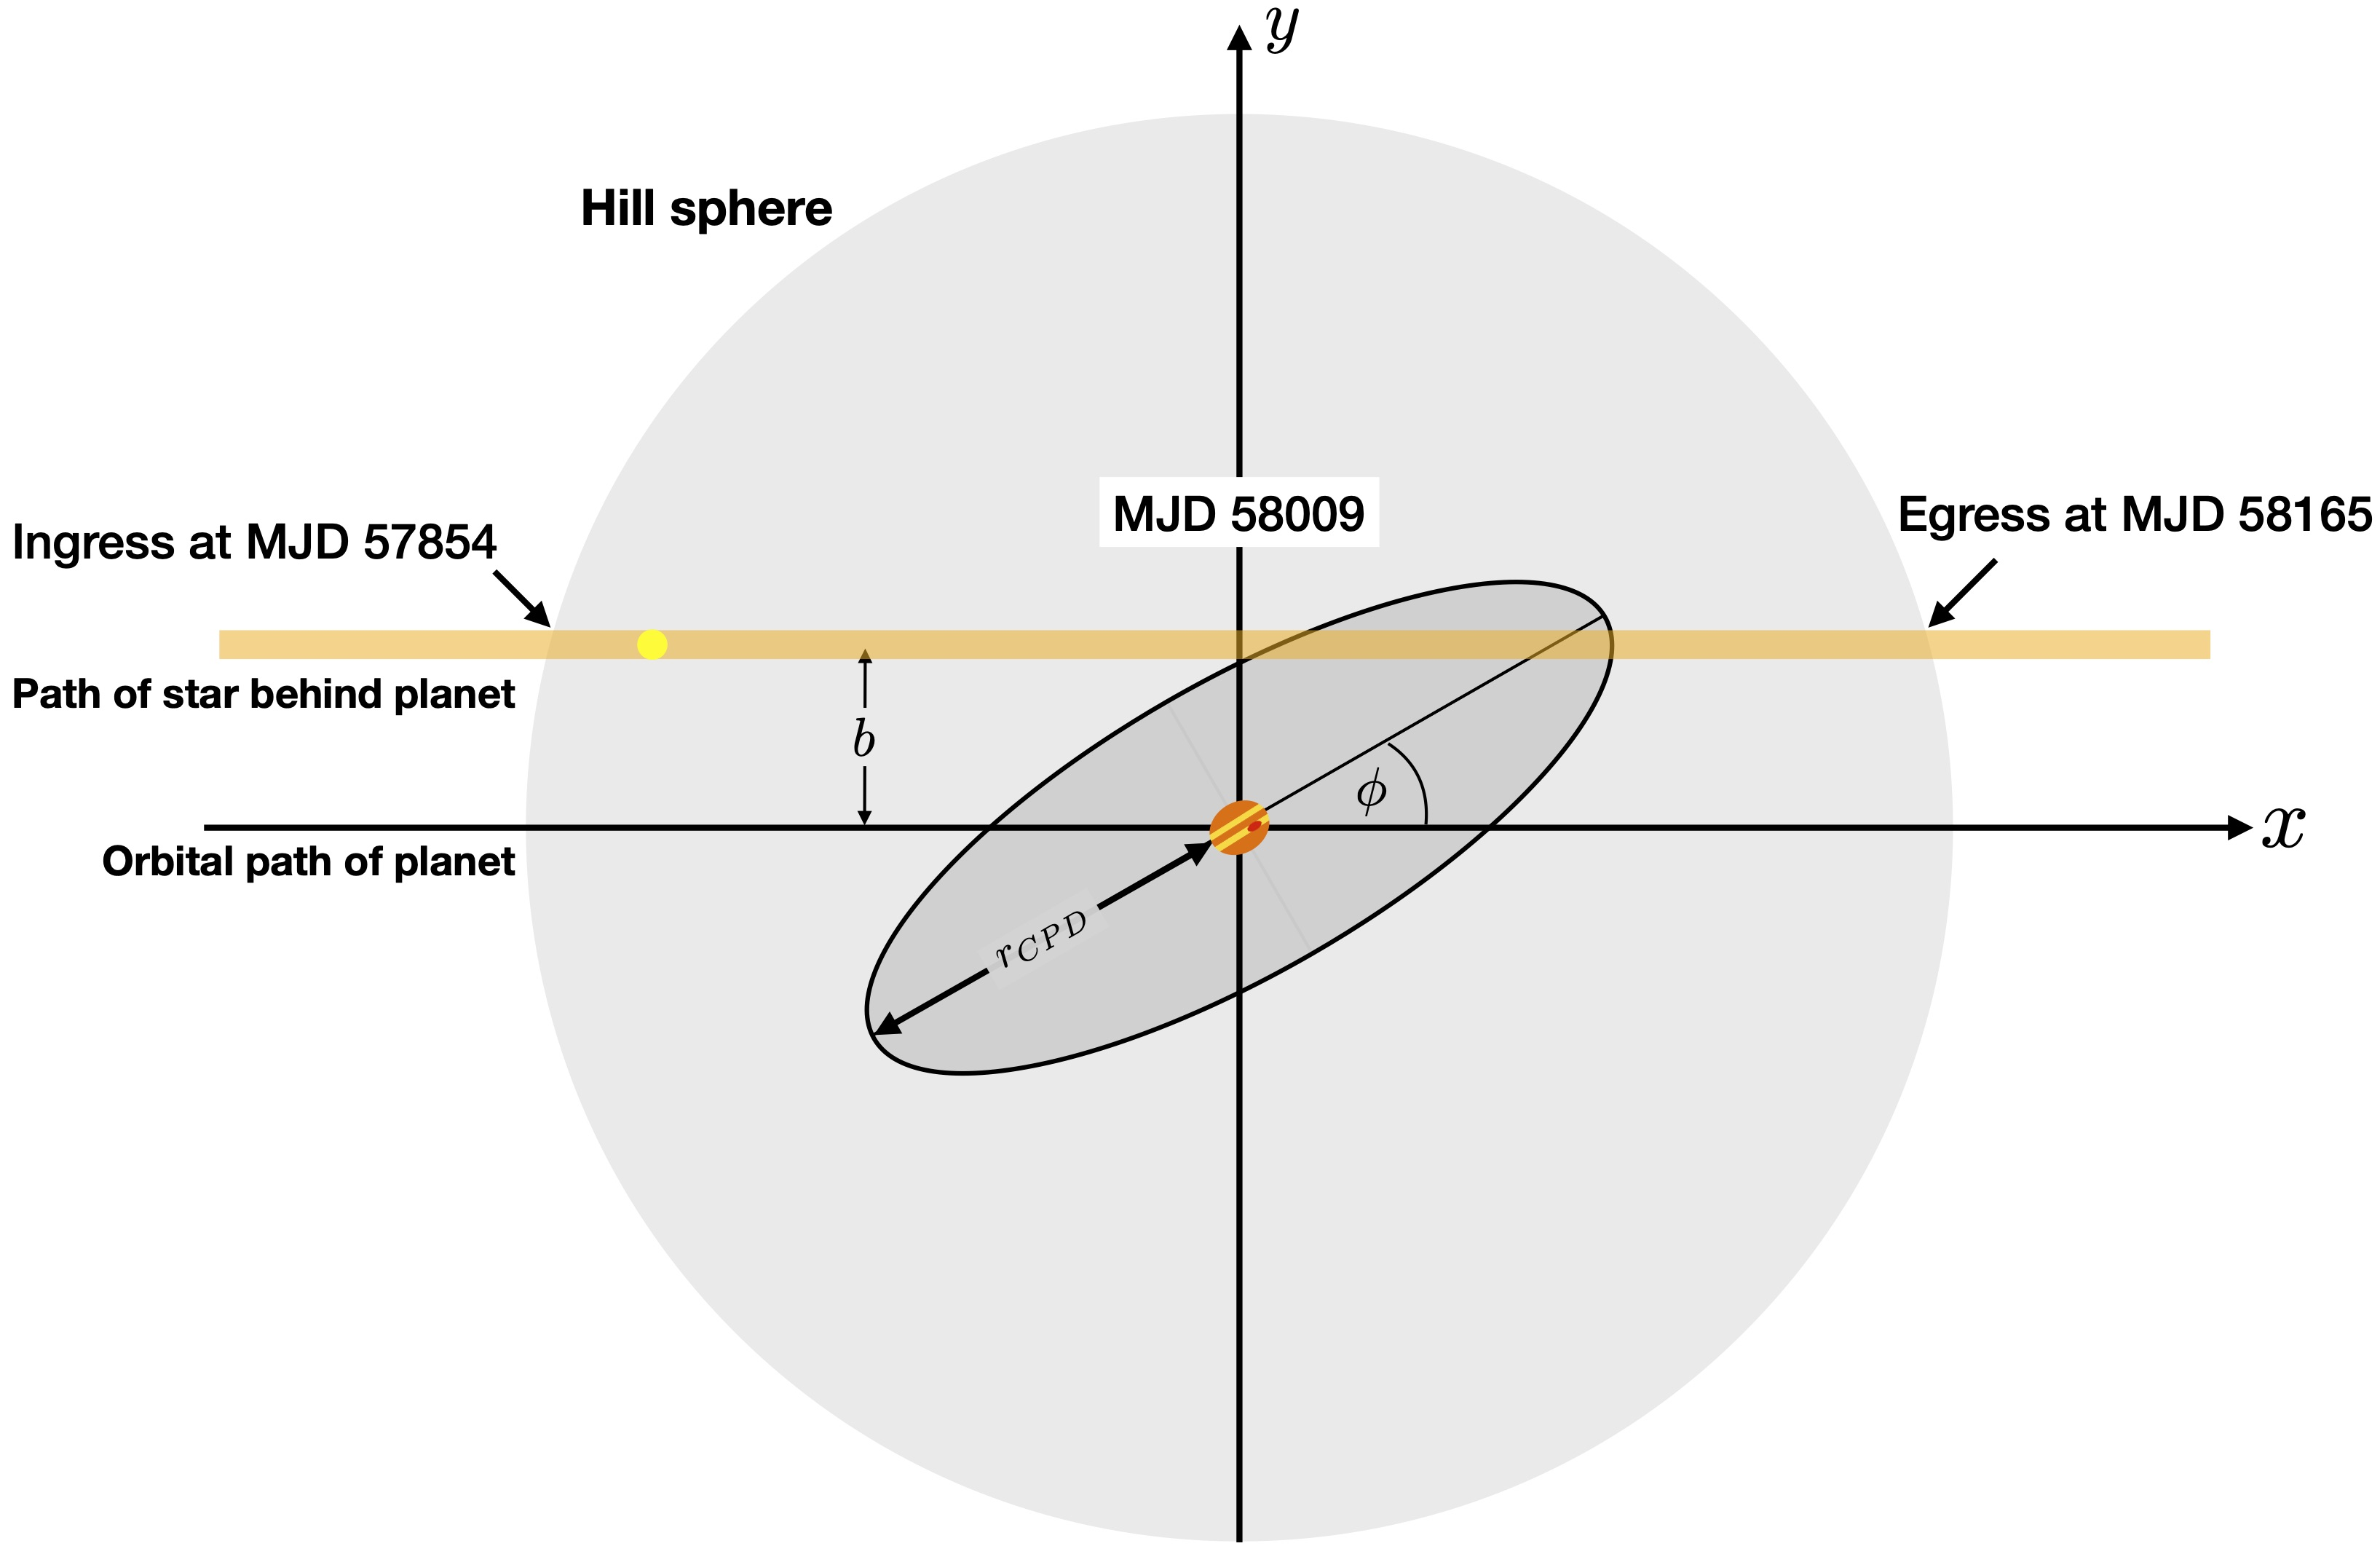
\includegraphics[width=0.8\textwidth]{disk_sketch.jpg}
\caption{Sketch of the CPD model showing how the coordinate system and orientation of the CPD is defined. The star moves on the defined path behind the Hill sphere and the CPD.}
\label{cpdmodel}
\end{figure*}

The reduction steps for each telescope are detailed in the sections below.
%
To reduce the size of the photometric datasets, we took a binned average of 0.05 days (72 minutes) for bRing, ASTEP, and BRITE.
%
The photometric series from the four telescopes are shown in Fig.~\ref{fig:binnedphot}.

\subsection{bRing and MASCARA}

Monitoring the Hill sphere transit of \bpb{} for several months requires multiple dedicated observatories distributed in longitude.
%
To this end, the bRing observatories \citep{Stuik17} were built and deployed to Sutherland, South Africa, and Siding Springs, Australia.
%
The first bRing observatory was built and tested at Leiden Observatory (PI: M. Kenworthy) and deployed almost exactly one year after the initiation of the project, with first light on 2017 January 6 at the South African Astronomical Observatory in Sutherland, South Africa; the details of the completely automated observatories are detailed in \citet{Stuik17}.
%
The second bRing observatory was built at the University of Rochester and deployed by S.~Mellon and E.~Mamajek to Siding Springs, Australia \citep{Mellon20Thesis}.
%
These observatories were based on the design of and the experience gained with the MASCARA observatories at Leiden Observatory  \citep{talens2017}, with the aim of producing accurate photometry of the brightest stars ($m_V\ < 8.4$).
%
The cameras do not have a filter in front of them, leading to an effective bandpass from 463nm to 639nm.
%
The bRing camera pixels are approximately 1 arcminute per side, and the commercial photographic camera lenses used have a \ac{psf} that changes shape and size significantly across the field of view.
%
The cadence of bRing observations is one image every 12.8 seconds.
%
A custom pipeline \citep{talens2018} was written to take the bRing data and produce photometry with 1\% precision.
%
Although the two bRing observatories had almost complete longitudinal coverage for \bp{}, additional data were gathered from MASCARA-South, at La Silla Observatory, Chile, to enable redundant observations.
%
With a maximum observable zenith angle for the bRing stations of $\approx 80\deg$, \bp{} remained visible for at least 1 hour per night all year round.
%
During the Hill sphere transit itself, bRing took 9528 binned data points and each camera averaged 108 binned data points per night.


MASCARA and bRing are ground-based observatories that use stationary, wide field cameras.
%
The data show strong trends introduced by inter-pixel sensitivity variations, lens transmission, atmospheric transmission and weather, and light contamination from the Sun, moon, and neighbouring stars.
%
For the calibration and detrending, a two-step approach was used.
%
The initial calibration was performed according to the steps described in \citet{talens2018}.
%
This calibration performs a spatiotemporal calibration based on the average behaviour of all stars in the camera's field of view, over a baseline of approximately two weeks, and removes most of the spatial variation signatures in the PSF and transmission, the variations in inter-pixel sensitivity, and the variations in the atmospheric transmission due to clouds or dust.
%
The residual systematic trends in the data vary from star to star, both on daily timescales and on monthly and yearly timescales, and are attributed to the sub-Nyquist sampling of the camera \ac{psf} by the lenslet array fixed on the interline readout Complementary Metal Oxide Semiconductor (CMOS) array.
%
\citet{talens2018} describes several models for these individual trends in the data and their subsequent removal.
%
Here we used a modified approach of the `local-linear' method, where instead of fitting the sky background, we fitted the moon phase and altitude and used them as an estimate for the sky background.
%
Similar to \cite{talens2018}, we iteratively solved with a three-day moving mean to separate trends from the daily variability.
%


\begin{figure*}[htb]
\centering
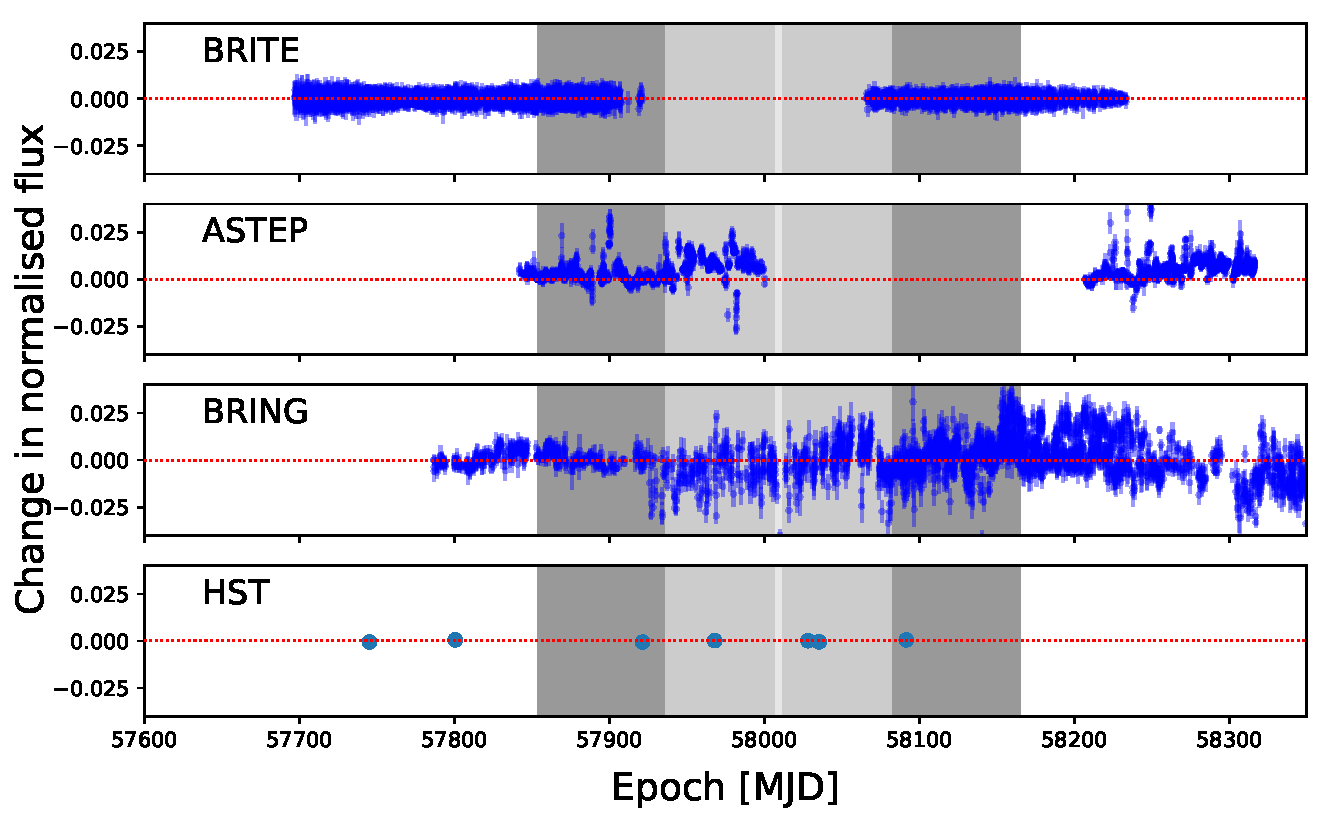
\includegraphics[width=1.0\textwidth]{all_binned_photometry.pdf}
\caption{Binned photometry of \bp{} for the four observatories. The transit of the Hill sphere of \bpb{} is shown as light grey and dark grey panels, representing the 100\% and 50\% radii of the Hill sphere, respectively, and the midpoint is the closest approach.}
\label{fig:binnedphot}
\end{figure*}

It is clear that there are residuals on timescales of hours to days with amplitudes of up to 3\%.
%
When all three telescopes show photometric data, we see that the photometry from two of the three telescopes sometimes agrees, with the third showing a deviation of up to 2\%.
%
We infer that these are due to systematics within that given telescope and not due to astrophysical phenomena associated with the \bp{} system.

\subsection{BRITE-Constellation}

BRITE-Constellation\footnote{\url{https://brite-constellation.at/}} is a set of five nanosatellites each with a 3cm diameter telescope re-imaging onto an uncooled Charge Coupled Device (CCD) \citep{Weiss14}.
%
Three of the satellites -- BRITE-Toronto (BTr), Uni-BRITE (UBr), and BRITE-Heweliusz (BHr) -- observe with a red filter (550-700nm) and two -- BRITE-Austria (BAb) and BRITE-Lem (BLb) --  observe with a blue filter (390-460 nm). \citet{pablo2016} includes a detailed description of the detectors as well as of pre-launch and in-orbit tests.
The data are reduced with a custom pipeline \citep{Popowicz17} that processes the observed images and produces instrumental magnitudes that are delivered to the users.
%
The satellites observe a 24 square degree wide field of view that contains 15-20 bright $(V<6)$ stars and at least three targets brighter than $V=3$ mag. Each field is observed for at least 15 minutes in each $\sim 100$ min orbit for up to half a year.
%
Beta Pictoris was observed during three consecutive seasons with the BRITE-Constellation nanosatellites:
The first observations of \bp{} were obtained
from UT 2015 March 16 to UT 2015 June 2 (BRITE Run ID: 08-VelPic-I-2015), yielding a total time base of 78.323 d using the BHr (red filter) satellite.
%
Second and third observing runs were conducted using BTr (red filter) from
UT 2016 November 4 to UT 2017 June 17,
% 4 November 2016 to 17 June 2017
for a total of 224.573 d, and using BLb (blue) from
% 15 December 2016 to 21 June 2017
UT 2016 December 15 to UT 2017 June 21 for 187.923 d
(BRITE Run ID: 23-VelPic- II-2016).

BRITE-Heweliusz was used from UT 2017 January 7 to UT 2017 January 30
% 7 January 2017 to 30 January 2017
for 24 days to cover a gap in the BTr observations.
%
During the third season, the red filter BHr satellite obtained time series of \bp{} between
% 9 November 2017 and 25 April 2018
UT 2017 November 9 and UT 2018 April 25, for 167.335 days
(BRITE Run ID: 33-VelPicIII-2017).
%
The BRITE-Constellation data of \bp{} are publicly available in the BRITE Public Data Archive\footnote{\url{https://brite.camk.edu.pl/pub/index.html}}.
%

In a next step, the raw photometric time series from the BRITE satellites were subsequently corrected for instrumental effects, including outlier rejection and both one- and two-dimensional de-correlations with all available parameters, in accordance with the procedure described by \citet{pigulski2018}.
%
A detailed description of the BRITE-Constellation data of \bp{} obtained during the three observing seasons and the corrections applied to them can be found in \citet{Zwintz19}.
%
In the present work, we used the same reduced and corrected light curves as in \citet{Zwintz19}. They are available on the CDS website\footnote{\href{http://vizier.u-strasbg.fr/viz-bin/VizieR?-source=J/A+A/627/A28}{http://vizier.u-strasbg.fr/viz-bin/VizieR?-source=J/A+A/627/A28}}.        

\subsection{ASTEP}

Photometric observations were conducted with ASTEP, a 40\,cm telescope installed at the Concordia station, Dome C, Antarctica.
%
ASTEP is a Newtonian telescope equipped with a five-lens Wynne coma corrector and a 4k $\times$ 4k front-illuminated Finger Lakes Instrumentation (FLI) Proline KAF-16801E CCD with 16 bit dynamic range.
%
The corresponding field of view is $1^\circ\times 1^\circ$ with an angular resolution of $0.93"\rm\ pixel^{-1}$.
%
The effective bandwidth of the instrument and telescope is from 575nm to 760nm \citep{Abe13}.

At the latitude of Concordia, $75^{\circ}.01$S, $\beta$\,Pic is circumpolar, allowing a continuous monitoring during the Antarctic winter season.
%
We observed it during two seasons, from
2017 March 5 to 2017 October 14 and from 2018 March 5 to 2018 July 16.
%
Data acquisition started automatically when the Sun was 8$^{\circ}$ below the horizon, with a 30 sec exposure when the Sun was between 6$^{\circ}$ and 8$^{\circ}$ below the horizon (dawn and twilight), and 60\,sec otherwise.
%
Because of $\beta$ Pic's brightness, we used a Sloan $i'$ filter ($0.695-0.844\,\mu m$) combined with a highly de-focused PSF of about 100 pixels in diameter.
%
We performed aperture photometry on the images, retrieving light curves for $\beta$ Pic and 17 comparison stars \citep[see][]{Mekarnia2017}.


The homogeneous set of light curves was in line with the excellent weather inferred from observations at Concordia between 2008 and 2012 \citep{Crouzet18}.
%
The $\delta$ Scuti variations are clearly visible in the day-to-day light curves \citep[][]{Mekarnia2017}.
%
The long-term stability of the light curves was, however, affected by two factors that were identified later.
%
First, the fact that $\beta$~Pic is about 13 times brighter than the first reference star implies that the correction for a varying background is less efficient than for usual observations of fainter stars \citep[e.g.][]{Mekarnia16}.
%
Second, snow storms led to the deposition of ice crystals not only on the primary mirror, but also on the entrance window to the camera box, in a region where the optical rays are not parallel.
%
This led to global changes in the photometry of the target and reference stars depending on where ice was deposited on the entrance window and on the location of the stars in the sky.
%
For MJDs before 57970, HD~38891 ($\alpha$\,=\,05:46:11.9, $\delta$\,=\,-50:52:18; J2000) was utilized to calculate the daily median used to calibrate the data over a given night.
%
After a snow storm that introduced vignetting on MJD 57970, HD~38891 was used with a multiplicative factor of 0.985 up to MJD 57907.
%
A subsequent removal of ice crystals after MJD 57907 changed the stability of the photometry, and HD~38745 ($\alpha$=05:45:11.7, $\delta$=-50:56:59)
 was used for calibration after this date.
%
Only photometry with the Sun more than 15 degrees below the local horizon was used ({\tt SUNELEV} $<-15^{\circ}$); data that are flagged as photometrically poor as well as any observations where the sky background rises above 200 counts were removed.


\subsection{Hubble Space Telescope}

Two \ac{hst} programmes (GO-14621 and GO-15119; PI: Wang) obtained precision photometric data using the ultraviolet imaging spectrograph (UVIS) on Wide Field Camera 3 (WFC3) in spatial scanning mode.
%
In the first programme, we monitored the flux of \bp{} over four visits within a span of 8.5 months (UT 2016 December 22, UT 2016 February 16, UT 2016 June 16, and UT 2017 August 2).
% and Feb. 16, June 16, Aug. 2, 2017).
%
The first two visits were timed to acquire a baseline (out-of-transit) constraint, and the final two visits were timed to coincide with the predicted full Hill sphere ingress and transit.
%
We acquired two \ac{hst} orbits per visit in order to effectively model the star's variability.

The second programme consisted of three visits spanning just over two months (UT 2017 October 1, UT 2017 October 8, and UT 2017 December 4).
% (Oct. 1, Oct. 8, Dec. 4, 2017).
%
These visits were timed to obtain precise constraints during the half and full Hill sphere egress.
%
For this programme, we only acquired one \ac{hst} orbit per visit because we found that the visit-to-visit variability during the first programme was larger than the star's variability within a given visit.

We used WFC3's UVIS detector in 2K2C sub-array mode (2k$\times$2k pixels, amplifier C) with the F953N narrow-band filter (953~nm).
%
For each frame, we scanned the star along the $x$ axis at a rate of 0.5\arcsec\,s$^{-1}$
% arcsec/sec
for 110 seconds, thus spanning $\sim$1400 pixels per frame.
%
The Space Telescope Science Institute recommends scanning in both forward and reverse directions to ensure that the target returns to the same point on the detector during each subsequent scan.
%
We performed at least five round-trip scans per \ac{hst} orbit; orbits with guide star re-acquisitions permitted an additional forward scan.  All seven visits within both programmes used this observing setup.

\begin{figure*}
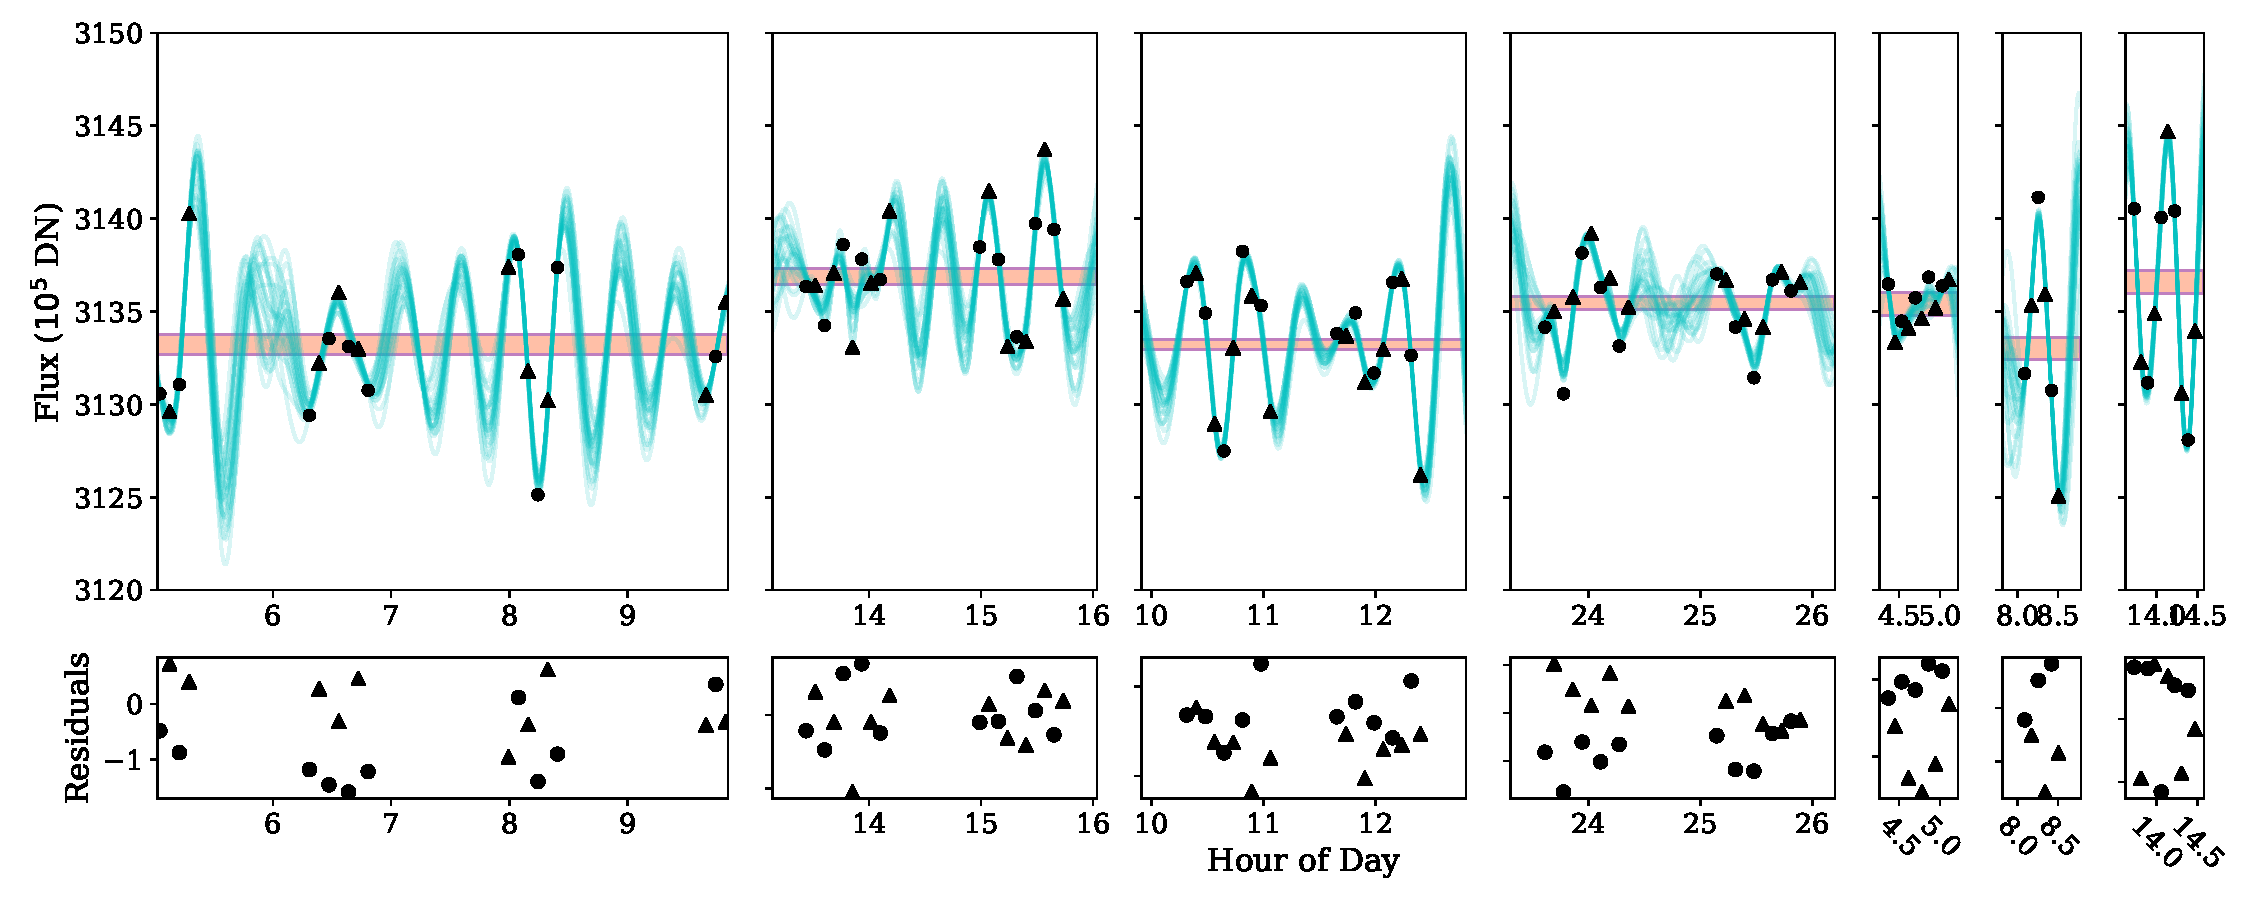
\includegraphics[width=1.0\textwidth]{hst_visitall-gpfit-maternperiodic.pdf}
\caption{\ac{hst}/WFC3/UVIS spatial scanning photometry obtained from all seven visits. The top panels show the data and model fits at each epoch. The forward scans are plotted as black circles. The reverse scans are plotted with black triangles and have been scaled to correct the offset between the two scan directions. The teal lines are Gaussian process models of the photometry using Gaussian process parameters drawn randomly from our Markov chain Monte Carlo analysis. The horizontal red line represents the 1$\sigma$ statistical uncertainty on the flux level in each of the visits and does not include the uncertainty of the photometry between visits. The bottom row shows the average residuals to the fits.
\label{fig:visits}}
\end{figure*}

We used a custom pipeline to extract the time-series photometry from the WFC3/UVIS data.  Originally written for WFC3 infrared analyses \citep[e.g.][]{Stevenson2014a, Stevenson2014c}, the pipeline uses standard data reduction techniques that were optimized for this particular observation.  For our final solution, we extracted a 1500 $\times$ 700 pixel region centred on the scanned star, utilized a 1500 $\times$ 100 pixel rectangular aperture to determine the stellar flux, and used the remaining region for background subtraction.
%
The raw photometry from WFC3/UVIS contains a clear offset between the flux measured from the two spatial scanning directions.
%
We have assumed in this analysis that it differs by a multiplicative scale factor.
%
Given the known $\delta$ Scuti pulsation periods between 30 and 60 min \citep{koen2003a, koen2003b} and the sparse time sampling but high precision of these \ac{hst} data, it is unfeasible to fit the over 30 known pulsation modes and it is not useful to use previous measurements of the pulsation that do not characterize the pulsations at sufficient precision \citep{Mekarnia2017}.


We are ultimately interested in the average flux for each visit.
%
Since each visit lasts multiple hours, we sampled over a full period of $\delta$ Scuti pulsations and thus retrieved the average flux value.
%
Adapting a similar approach as \citet{Johnson2015}, we modelled the stellar activity as a Gaussian process.
%
As we did not have sufficient cadence to sample the oscillations, we treated the $\delta$ Scuti pulsations as a quasi-periodic Gaussian process, where the periodic term roughly describes the strongest pulsation mode, and the `quasi' term accounts for the fact the modes constructively and destructively interfere, causing the amplitude to change over time.
%
We parameterized the quasi-periodic kernel as the product of a Mat\'ern kernel and a periodic kernel:

\begin{equation}
 K_{ij} = A^2 \cos\left(2\pi t_{ij}/P_{osc}\right) (1 + \sqrt{3}t_{ij}/l) \exp\left(-\sqrt{3}t_{ij}/l\right).
\end{equation}

Here, indices $i$ and $j$ refer to two data points separated in time by $t_{ij}$.
%
We have assumed that times between visits are so far apart that there is no correlation, but we have also assumed that they are drawn from the same Gaussian process. The $P_{osc}$ is roughly the period of the dominant pulsation mode, and $l$ is the covariance length that damps correlation at long time baselines, making the kernel quasi-periodic.

We have assumed that all seven epochs have $\delta$ Scuti pulsations that can be modelled by the same Gaussian process and that the flux offset between the two scan directions is the same multiplicative factor.
%
Running the following analysis on each individual visit did not indicate that any of these parameters were different.
%
We ran a Bayesian parameter estimation to fit for the flux in all seven epochs as well as the three Gaussian process parameters ($A$, $P_{osc}$, and $l$) and the multiplicative factor to correct for the offset between the scan directions.
%
We also fitted for a term that increases the error of each flux measurement above the nominal photon noise term to account for unknown effects, such as the imperfection of the Gaussian process kernel in fully modelling the observed stellar activity.
%
We used uniform priors on the flux at each epoch and log-uniform priors on all of the nuisance parameters.
%
We used \texttt{emcee} \citep{ForemanMackey13} to sample the posterior of fluxes, marginalizing over all nuisance parameters.
%
The Gaussian process regression was implemented with our own custom code.

Looking at the nuisance parameters, we find a multiplicative scale factor of $0.9984 \pm 0.0001$ for the fluxes from the second scan direction.
%
Our Gaussian process finds a period of $29.3 \pm 0.8$~minutes, which is slightly smaller than all of the known pulsation periods.
%
This shorter period might allow the Gaussian process model to fit the full range of pulsation frequencies best.
%
We found that we needed to scale the uncertainties on the photometry of each scan by $1.9 \pm 0.1$ times the photon noise limit to account for the scatter in our measurements.
%
It is difficult to determine whether the additional noise above the photon noise floor is due to the instrument, data reduction, or the Gaussian process not being a perfect model of the pulsations.
%
The HST data and the Gaussian process model used to measure the average flux in each epoch are shown in Fig.~\ref{fig:visits}.

The statistical uncertainty on the flux in each epoch from our analysis is 0.01--0.02\%.
%
However, comparing the two out-of-transit observations, we find a difference of 0.11\%, which is likely limited by the stability of the telescope between visits.
%
This is consistent with a finding of 0.1\%  repeatability for UVIS drift scans by the instrument team \citep[Instrument Science Report WFC3 2017-21;][]{Shanahan2019}.
%
It is therefore reasonable to expect a similar amplitude of uncertainty during all in-transit visits, and we used 0.06\% as our 1$\sigma$ uncertainty in the flux of each epoch.
%
Unlike typical exoplanet transit observations with the \ac{hst}, where the out-of-transit and in-transit photometry can be obtained in the same visit, we relied on the photometric stability from visit to visit.

Due to the uniqueness of the transit, we would have followed up on anything with greater than a 3$\sigma$ deviation from the out-of-transit flux.
%
However, we did not observe the star to dim significantly during any of our visits, so we established the 3$\sigma$ value of 0.18\% as our sensitivity limit.

\subsection{Summary of photometric data}

The photometric measurements from the HST suggest that there were no significant variations in the photometry of \bp{} at the times of the seven visits.
%
In each of the two separate seasons of BRITE photometry, no long-term variation is seen.
%
The HST shows that there is no relative offset between the BRITE seasons, implying that there was no long-term astrophysical variation during the observations from the space-based observatories.
%
%HST confirms the photometry of BRITE, and the two separate seasons of BRITE photometry shows no long term variations in the brightness of Beta Pictoris.
%
The HST and BRITE therefore provide a check of the variations in the photometry seen in the bRing and ASTEP data during the Hill sphere transit, where we see larger variations.
%
We therefore hypothesize that any possible astrophysical fluctuations in the ground-based photometry are below the level introduced by time-varying systematic effects, which are of the order of 2\%.

\section{Analysis}\label{sec:analysis}

We searched for occulting material within the Hill sphere of \bpb{} by looking for long-term photometric changes as a function of the Hill sphere radius, with timescales of weeks to months.
%
Due to the difficulties of removing long-term systematics (and the danger of possibly removing any possible astrophysical signals), we hypothesize that there is no statistically significant \ac{cpd} detection with the BRITE photometry and that for parameter values outside of BRITE's coverage we can use the ground-based observatories to provide upper limits on $\tau$.
%
For this analysis, we studied the photometry from each telescope independently and then combined the results into a final sensitivity plot.

\subsection{Dust properties}\label{dust}

Our model derives limits on occulting material in terms of optical depth; to convert this into estimated limits on dust mass, we made some simple assumptions.
%
Using Eq. \ref{chen1}, we solved for the temperature of a dust grain ($T_{g}$) at a given distance $D$ from a source of temperature $T$ (in K) and radius $R$ \citep{Chen01}:

\begin{equation}
\label{chen1}
T_{g} = \sqrt{\frac{R}{2D}}T
.\end{equation}
Using values from Table~\ref{bpicparams} yields an equilibrium temperature of $\sim$174 K due to stellar radiation and an equilibrium temperature of $\sim$101 K from the planet's thermal emission.
%
Even at a distance of 8.9\,au, the star's flux dominates that of the planet (the planet provides negligible heating beyond 0.01$r_H$). Ices will likely sublimate at these temperatures, so we adopted silicate as the dominant dust grain composition and adopted a density of $\rho_g$ = 2.5 g cm$^{-3}$, corresponding to the density of Jupiter's rings as measured by \citet{Chen01}.

Given the age of \bp{}, and the fact that the star itself has largely dispersed its primordial disk material, it is unlikely that any primordial gas-rich CPD has survived.
%
We have therefore assumed that any circumplanetary dust is replenished through collisions of larger objects and thus can be thought of (and modelled) as a microcosm of a circumstellar debris disk \citep[e.g.][]{Kennedy11}.
%
Typically, collisional dust-size distributions are such that most of the surface area is concentrated in the smallest surviving grains \citep{1969JGR....74.2531D}.
%
Thus, we estimated the minimum grain size for circumplanetary orbits using Eq. (9) of \citet{Kennedy11}; while this minimum size is analogous to the radiation pressure `blowout' size for circumstellar orbits, the smallest circumplanetary grains may also collide with the planet (or any moons) as their orbits are driven to high eccentricity \citep[see][]{Burns79}.
%
The true minimum grain size depends on the specific orbit, but this estimate is sufficient for our purposes here.
%
Assuming that dust is concentrated at the area-weighted mean planetocentric distance (0.7$r_{CPD}$; see below), the minimum size is $s = 31 \sqrt{r_{CPD}/r_{Hill}}$\,$\mu$m, approximately six times larger than the blowout size for circumstellar orbits.
% 2e5*sqrt(rCPD)*lstar/rho_kg_m3/mpl_earth^(1/3)/mstar^(2/3)


\subsection{Circumplanetary disk model}\label{mellonestimate}

The rings of the gas giant planets in the Solar System are perpendicular to the rotational axis of the parent planets, assembled there by the quadrupole moments of the planet's gravitational field.
%
At larger radii from a planet, it is expected that the rings become coplanar with the planet's orbit, and \citet{Speedie20} investigate the stability and extent of tilted ring systems around exoplanets.
%
A determination of the rotational period of \bpb{} (for example, by photometric monitoring) together with the radius of the planet would enable an estimate of the planetary obliquity projected onto the line of sight towards Earth.
%
The obliquity of \bpb{} is not known, although a measurement of rotational broadening by \citet{Snellen14} implies that the planet is not being viewed pole-on.
%
Given that the four gas giant planets in the Solar System have a range of obliquities from 3 degrees to 98 degrees, it is reasonable to assume that the obliquity of \bpb{} is unconstrained and that the angle between the rotational axis of the planet and its orbital plane is similarly unconstrained; however, it is worth noting that the spin axis of the star and the orbit of \bpb{} are co-aligned within measurement errors \citep{Kraus20}.
%
One might argue that any \ac{cpd} would be coplanar with the planet's orbital plane, but simulations by \citet{Martin20} show that \ac{cpd}s with small initial tilts can have their tilts increased via tilt instability, possibly moving them into our range of detection.
%
Once tilted, the stability of the inclined \ac{cpd}s from \citet{Speedie20} shows that they can last on long timescales and remain detectable in transit.
%
Coplanar \ac{cpd}s are truncated at 0.4\rhill{} \citep{Martin11}, but a tilted \ac{cpd} may have a larger truncation radius \citep{Lubow15,Miranda15}.
%
For the purposes of this analysis, we have assumed that a \ac{cpd} can be allowed at any orientation.

We constructed a simple model of the eclipse light curve for a CPD.
%
We have assumed that the disk has a height much smaller than its diameter, so we can approximate it as a thin slab of homogeneous material with a face-on optical depth $\tau$.
%
We used a coordinate system whose origin is the centre of the disk, with the positive $z$ axis pointing towards the observer.
%
The disk is circular, has a radius $r_{CPD}$, is centred on the origin, and initially lies on the xz plane.
%
It is inclined, rotating around the $x$ axis by $\theta$ degrees; it is then rotated around the $z$ axis by $\phi$ degrees in the direction from the positive $x$ axis towards the positive $y$ axis, as shown in Fig.~\ref{cpdmodel}.

The un-attenuated star flux has a value of $I_0$.
%
The starlight passing through the disk towards the observer is then attenuated as:

$$I=I_0 \exp (-\tau\sin \theta).$$

We have assumed that $\tau << 1$, and we Taylor-expanded the above equation to get

$$I = I_0(1-\tau\sin \theta),$$

which can be rearranged to get

$$\tau = \frac{(1-I/I_0)}{\sin \theta}. $$

The surface density of the disk $\sigma_{CPD}$ is given by $\tau/\kappa$. The total mass of dust in this disk is then

$$M_{CPD}=\frac{\tau}{\kappa} \pi r_{CPD}^2,$$

where $\kappa$ is the opacity in units of cm$^2$ g$^{-1}$ and can be written in terms of dust density $\rho$ and particle size $a$ as $\kappa=3/(4\rho a)$, leading to

$$M_{CPD}= \frac{4\tau a \rho}{3} \pi r_{CPD}^2.$$

The $x$ axis is parallel to the projected path of the star behind the disk, and the$ y$ axis is oriented such that the path of the star crosses the $y$ axis at impact parameter $b$ when $t = t_{b}$ at $x=0$.\ As such, the coordinates of the star at time $t_b$ is $(0,b)$ and the x coordinate at time $t$ is:

$$x_{star} = v(t-t_{b}).$$

In this way, we can calculate a model light curve $I(t)=f(r_{CPD},\tau,i,\phi,t_b,t)$.

For each instrument, we have the photometric time series $I(t)$ and the error on the measured flux $I_{err}(t)$.
%
We fixed the radius of the disk $r_{CPD}$ and generated a grid of trial values for the orientation of the disk in $(i,\phi)$.
%
With each pair of trial values, we calculated the reduced chi squared of the model with respect to the data, and we used the Python module {\tt lmfit} to perform the minimization and find the best fit $\tau$ value for the model.
%
An example disk and dataset are presented in Fig.~\ref{simdisk} for a disk with a radius 0.40\rhill{} and a best fit optical depth of 0.1, at an orientation $\theta=20^o, \phi=50^o$.
%
Contours of higher values of $\chi_{r}^2$ are not symmetric about the best fit but show narrow regions corresponding to disk geometries where the chord cut across the disk is of a similar length to the chord of the disk with the best fit.


%\begin{figure}[h]
\begin{figure}[htb]
    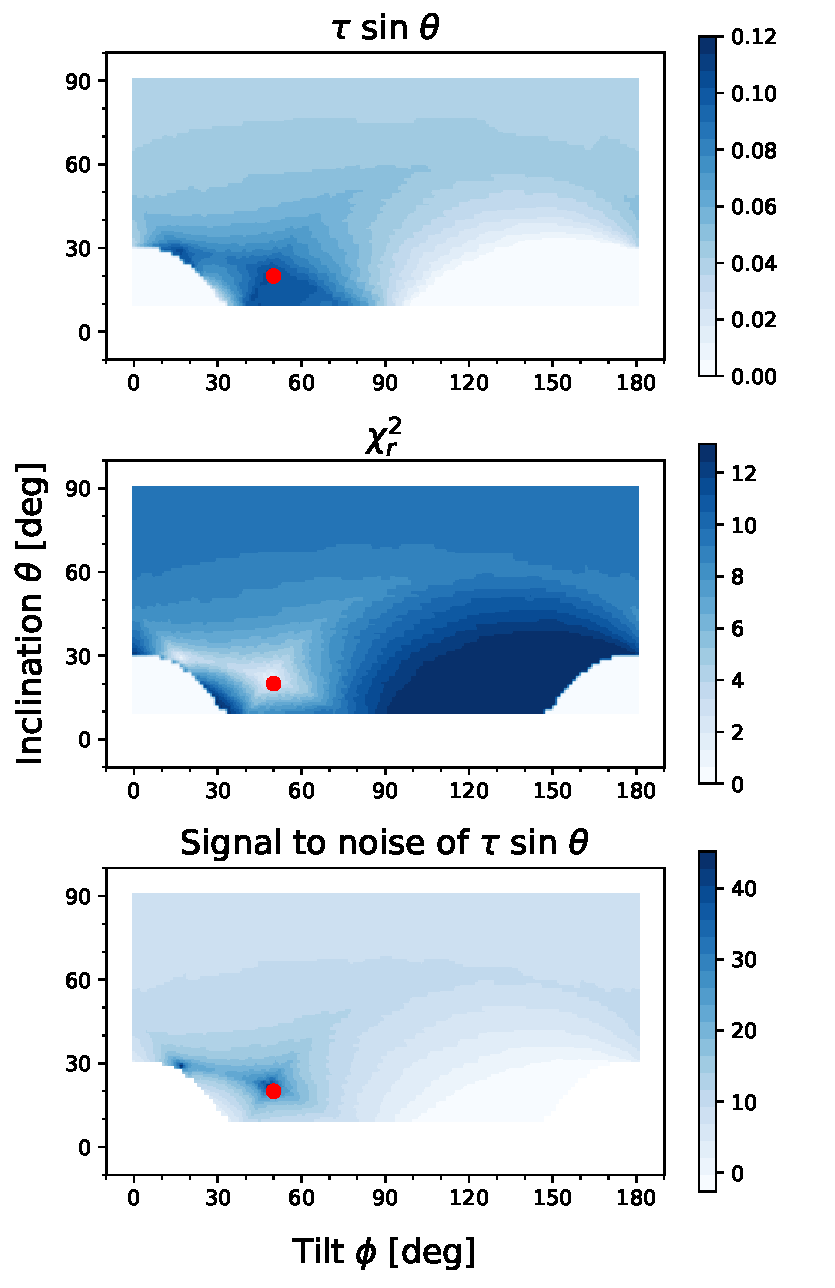
\includegraphics[width=\columnwidth]{simdisk_b.pdf}
    \caption{Fitting to a synthetic \ac{cpd} dataset showing the estimated $\tau$, the reduced chi squared, and the signal to noise of the measurement of $\tau$.
    %
    The red dot indicates the input inclination and tilt of the best fitting disk.}
    \label{simdisk}
\end{figure}


We produced maps of fitted optical depth $\tau$ for each of the three instruments and for two disk radii, 0.6\rhill{} (Fig.~\ref{cpd60}) and 0.30\rhill{} (Fig.~\ref{cpd30}).
%
Each of the observatories has a different temporal coverage of the transit, and so they probe different regions of parameter space for possible \ac{cpd} orientations.
%
The BRITE photometry shows no significant photometric systematics, while the two ground-based observatories, bRing and ASTEP, show significant non-zero values for $\tau$, represented as positive values of $\tau / \tau_\sigma > 1$ in the lower panels.
%
For a 60\% Hill sphere \ac{cpd}, we see that BRITE provides the most sensitive upper limits on the optical depth, but that bRing provides the most complete coverage of possible tilts and inclinations.
%
For the 30\% Hill sphere \ac{cpd}, the BRITE satellite coverage does not put any constraints on any possible \ac{cpd}s (see the light grey regions in Fig.~\ref{fig:binnedphot}).
%
The almost continuous coverage from bRing provides complete photometric coverage for smaller \ac{cpd}s, but at a cost of precision.

The long-term photometric monitoring places an upper limit on the mass of a \ac{cpd} around \bpb{} for geometries where a disk would intersect the chord drawn by the star behind the Hill sphere.
%
For a stable prograde (0.3\ \rhill{}) and retrograde (0.6\ \rhill{}) \ac{cpd}, the mass limits are $2.2\times 10^{21}$g and $1.8\times 10^{22}$g, respectively.
%
% For disk hill radius 0.60 we have an upper mass of 1.75e+22 g
% For disk hill radius 0.30 we have an upper mass of 2.22e+21 g
%%%This can be compared to the mass of dust determined from ALMA observations of $3\times 10^{24}$g

\begin{figure*}[htb]
    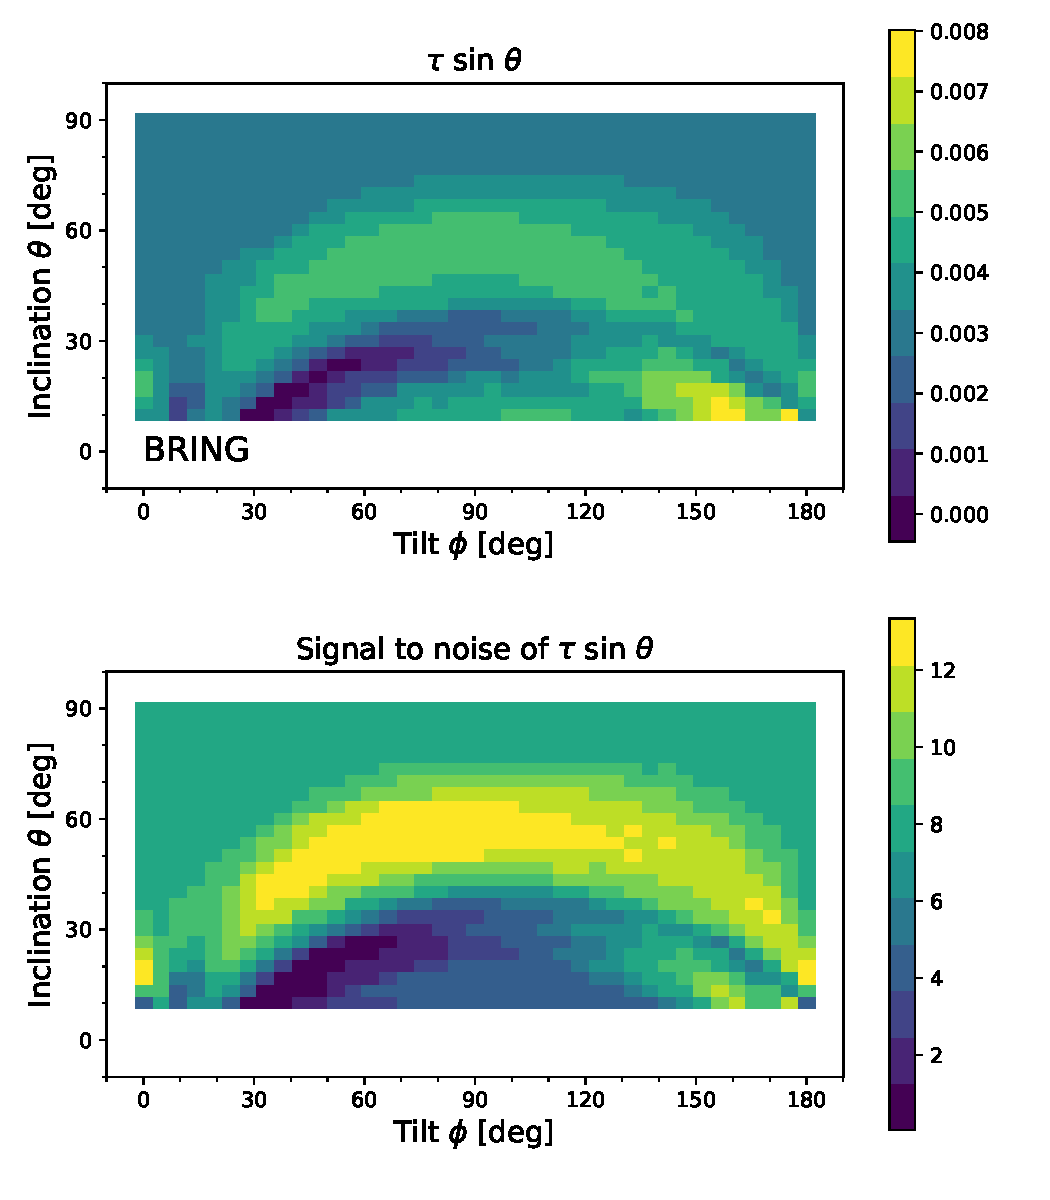
\includegraphics[width=0.333\textwidth]{diskfit_BRING_060.pdf}
%    \hfill
    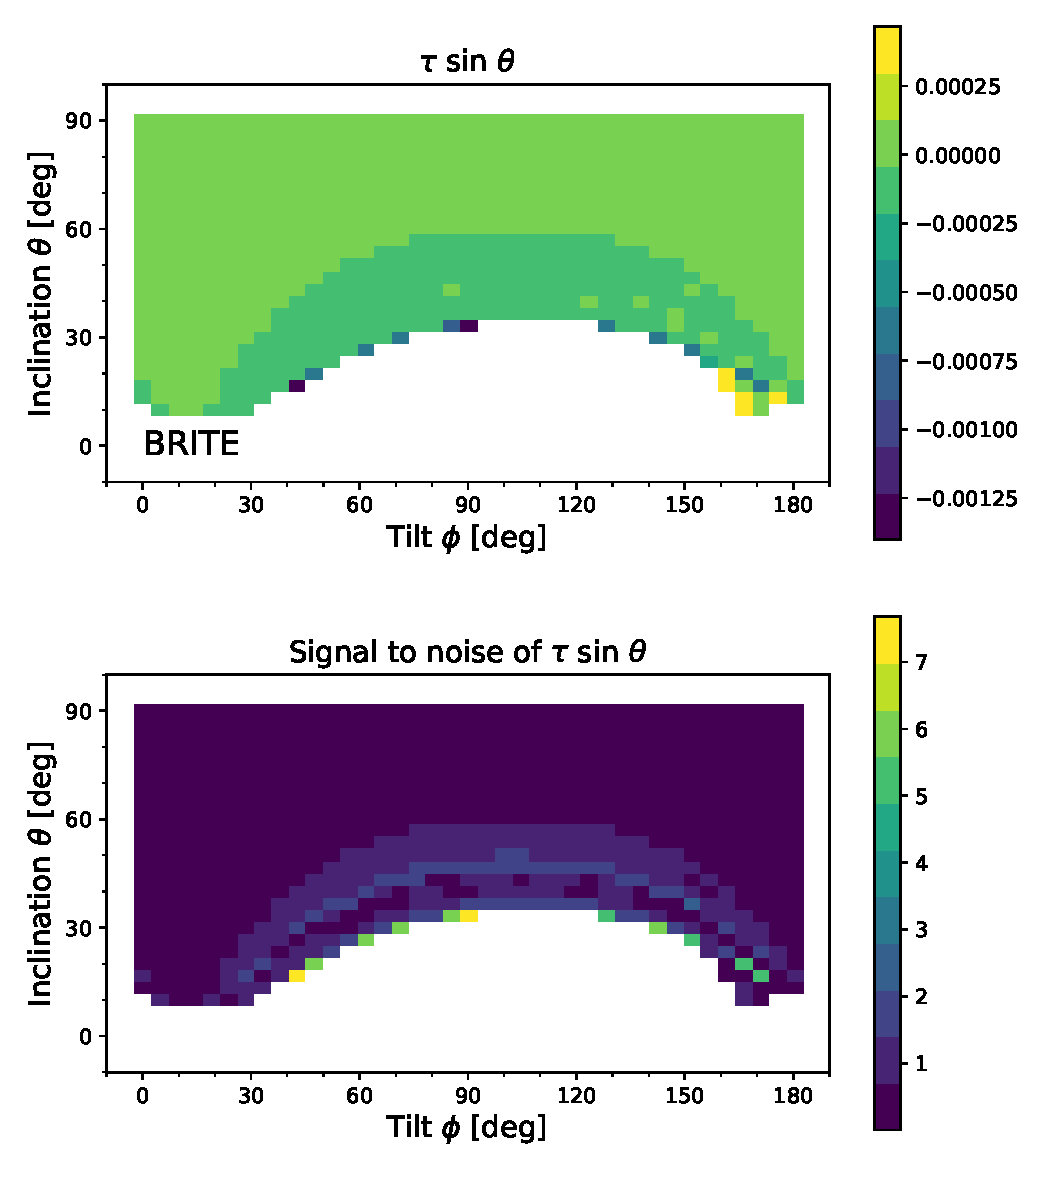
\includegraphics[width=0.333\textwidth]{diskfit_BRITE_060.pdf}
%    \hfill
    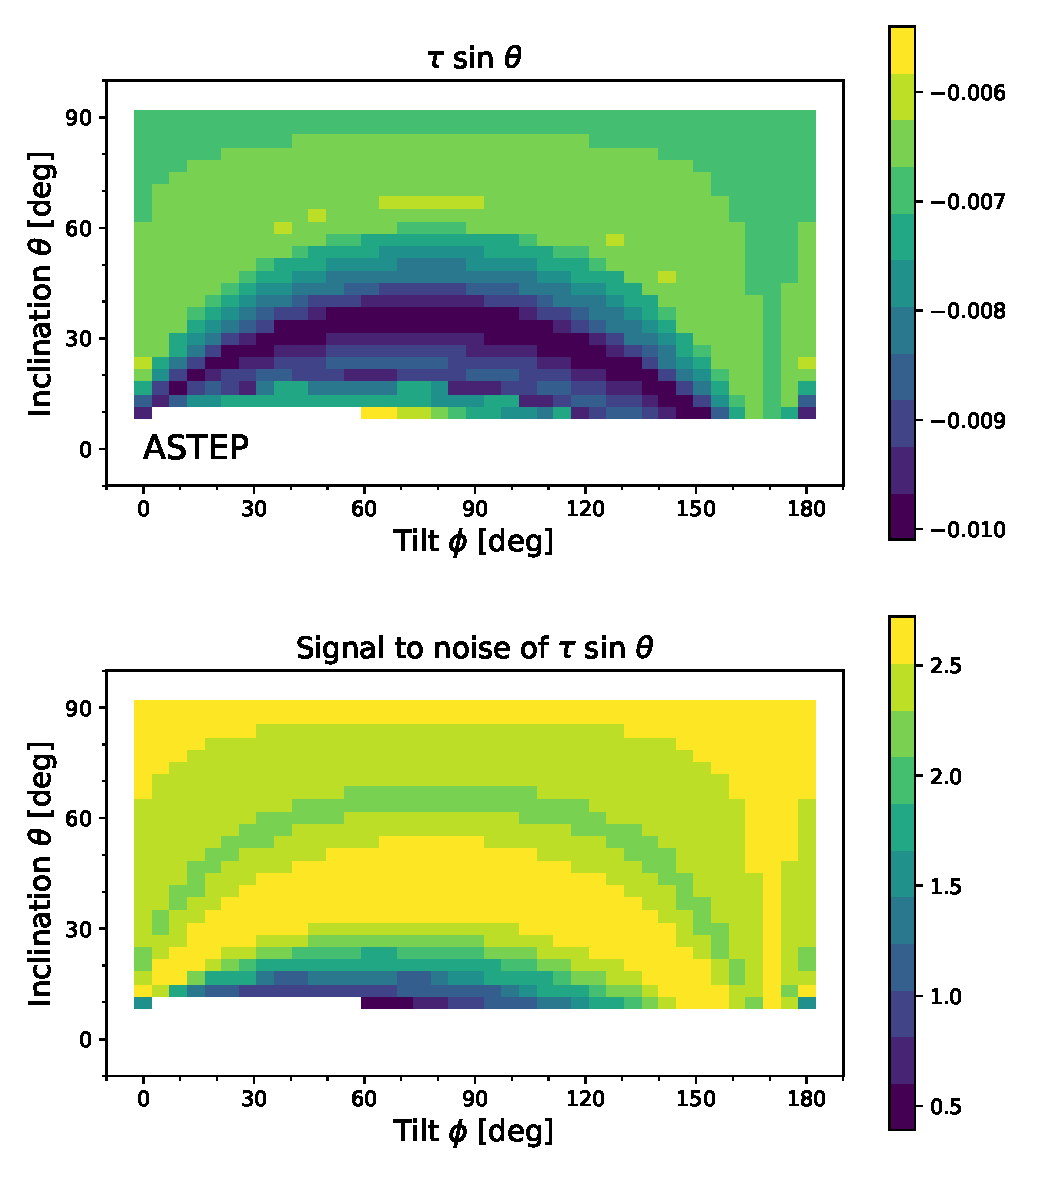
\includegraphics[width=0.333\textwidth]{diskfit_ASTEP_060.pdf}
    \caption{Circumplanetary disk fits for a disk with a radius of 0.60\ \rhill. The three observatories are shown in the three panels. The upper row of each panel shows the upper limit on the optical depth for a given tilt and inclination of the model disk. The numerical values of the upper limits are shown in the colour bars to the right of the plots. The white colour marks areas where there is no photometry with the given observatory to provide a constraint. The bottom row of each panel shows the signal to noise for each trial value of tilt and inclination.}
    \label{cpd60}
\end{figure*}

\begin{figure*}[htb]
    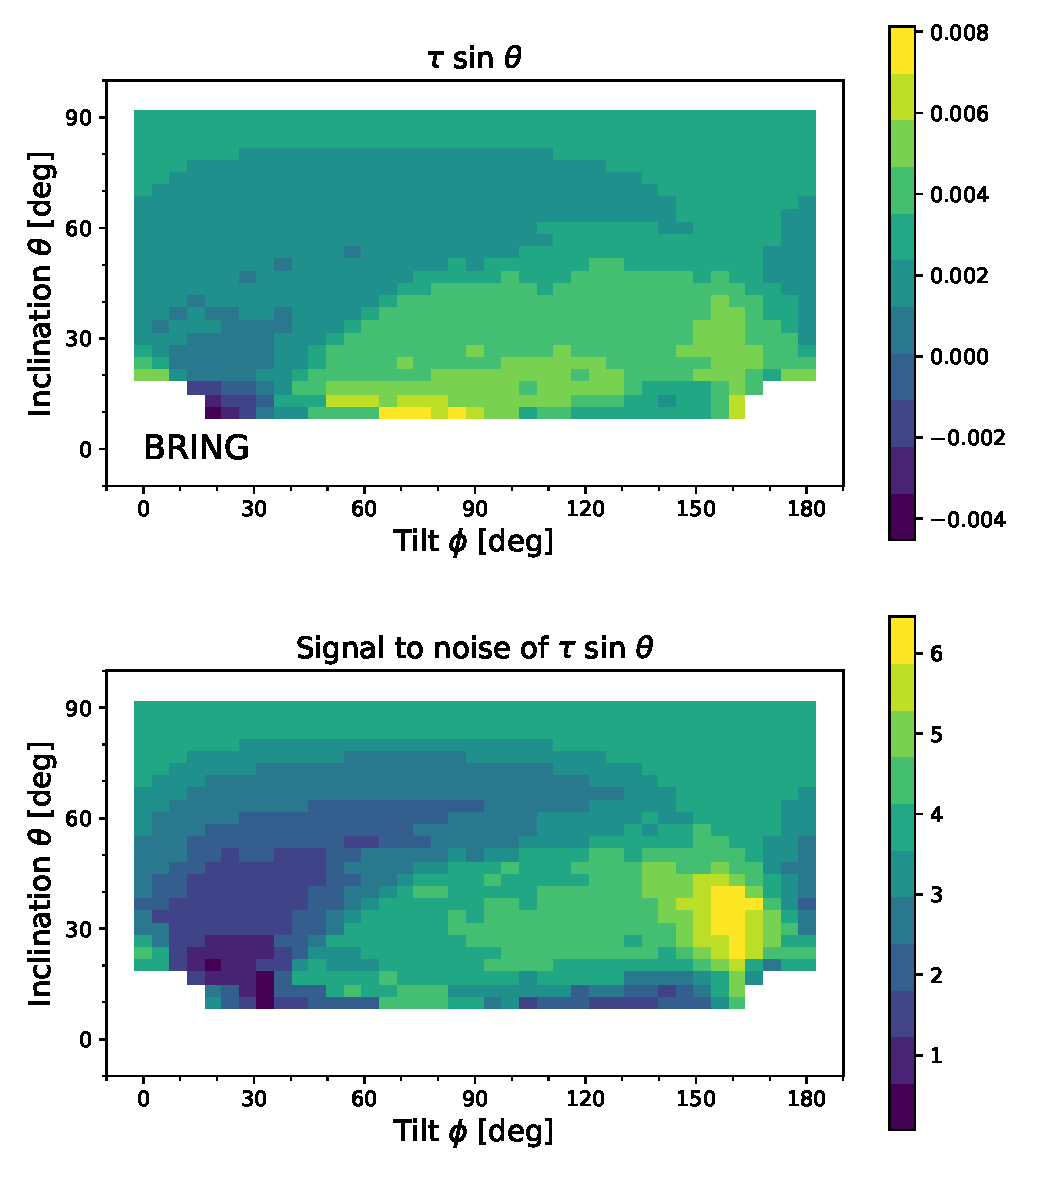
\includegraphics[width=0.33\textwidth]{diskfit_BRING_030.pdf}
%    \hfill
    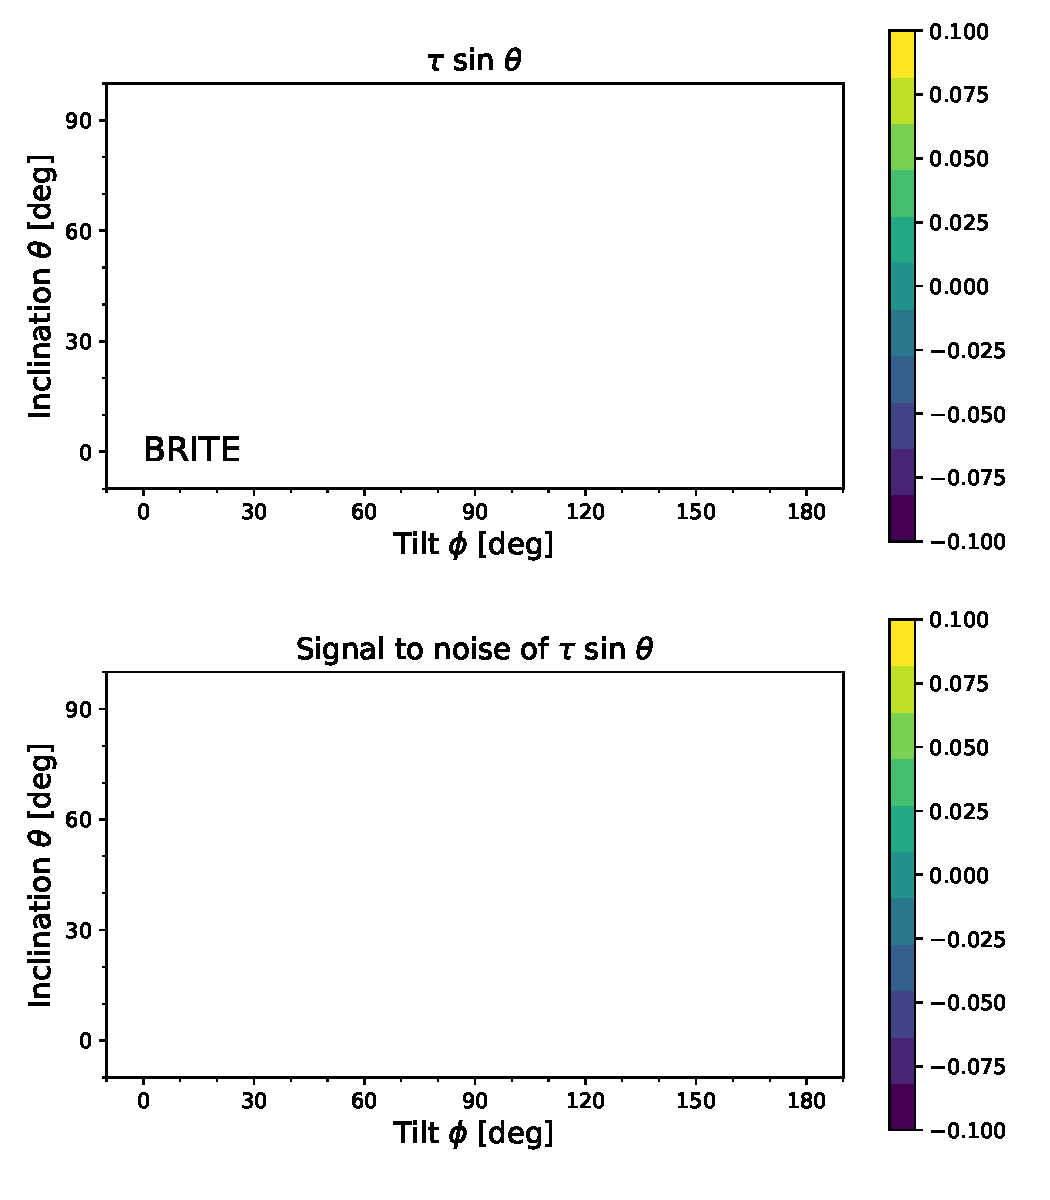
\includegraphics[width=0.33\textwidth]{diskfit_BRITE_030.pdf}
%    \hfill
    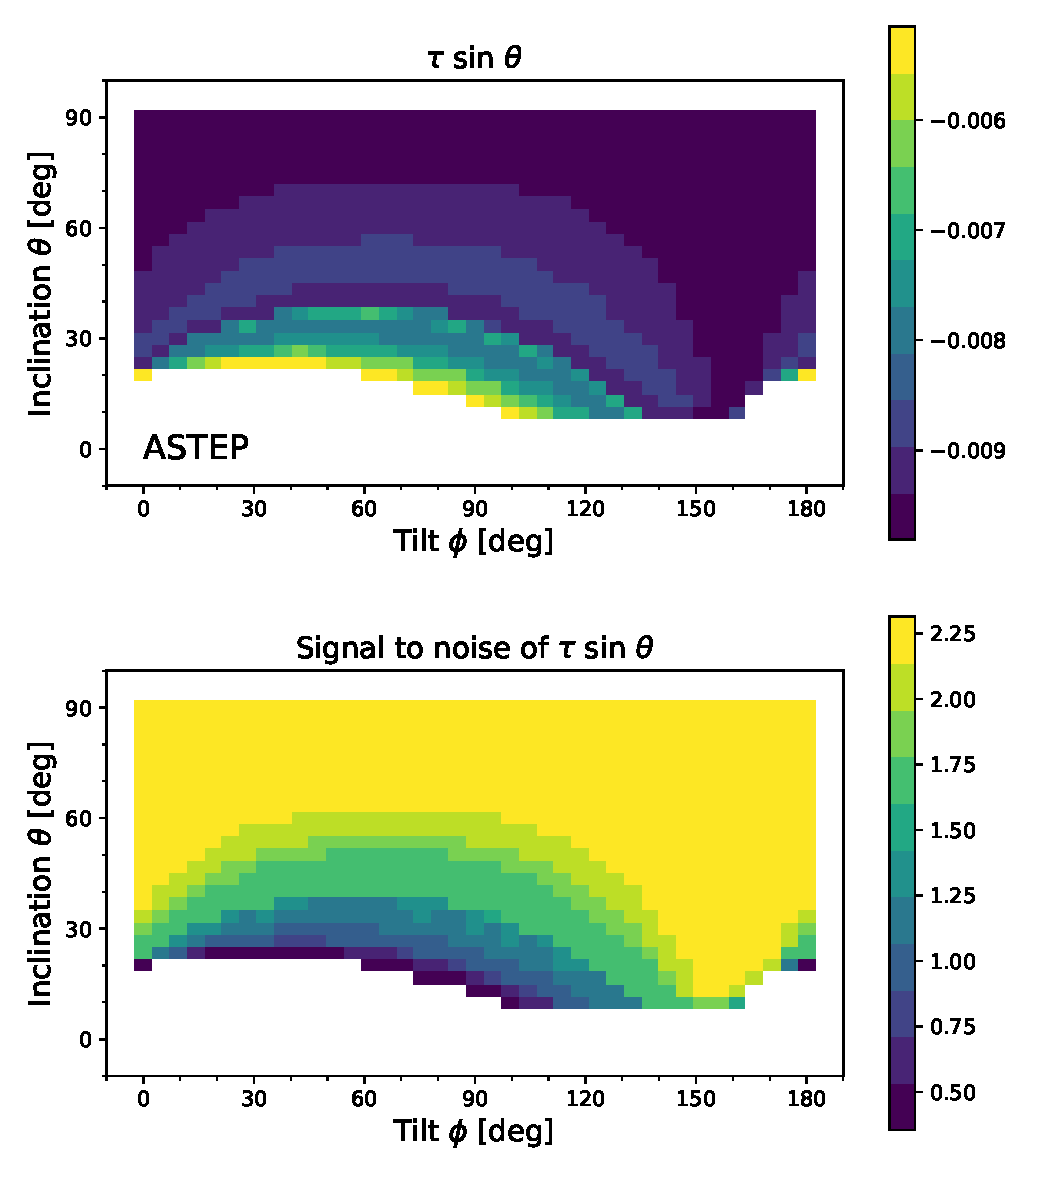
\includegraphics[width=0.33\textwidth]{diskfit_ASTEP_030.pdf}
    \caption{Circumplanetary disk fits for a disk with radius of 0.30\ \rhill. The three observatories are shown in the three panels in a similar format to Fig. \ref{cpd60}. The smaller radius for the CPD leads to different amounts of coverage within the tip and tilt parameter space. BRITE does not have photometric coverage to test any CPD model with a radius of 0.30\ \rhill.}
    \label{cpd30}
\end{figure*}

\begin{figure*}[htb]
    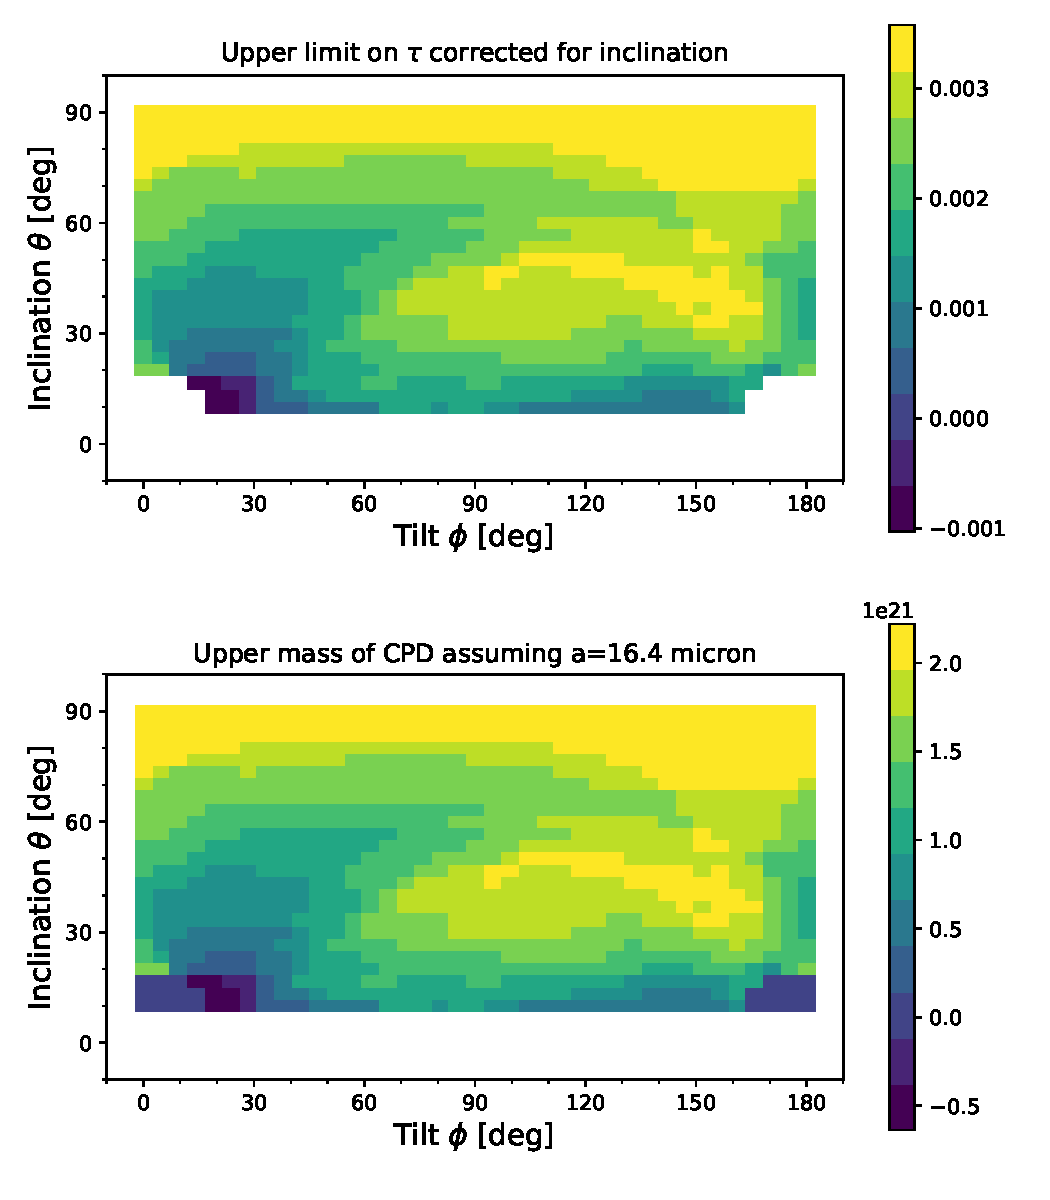
\includegraphics[width=0.50\textwidth]{diskfit_taumass_030.pdf}
%    \hfill
    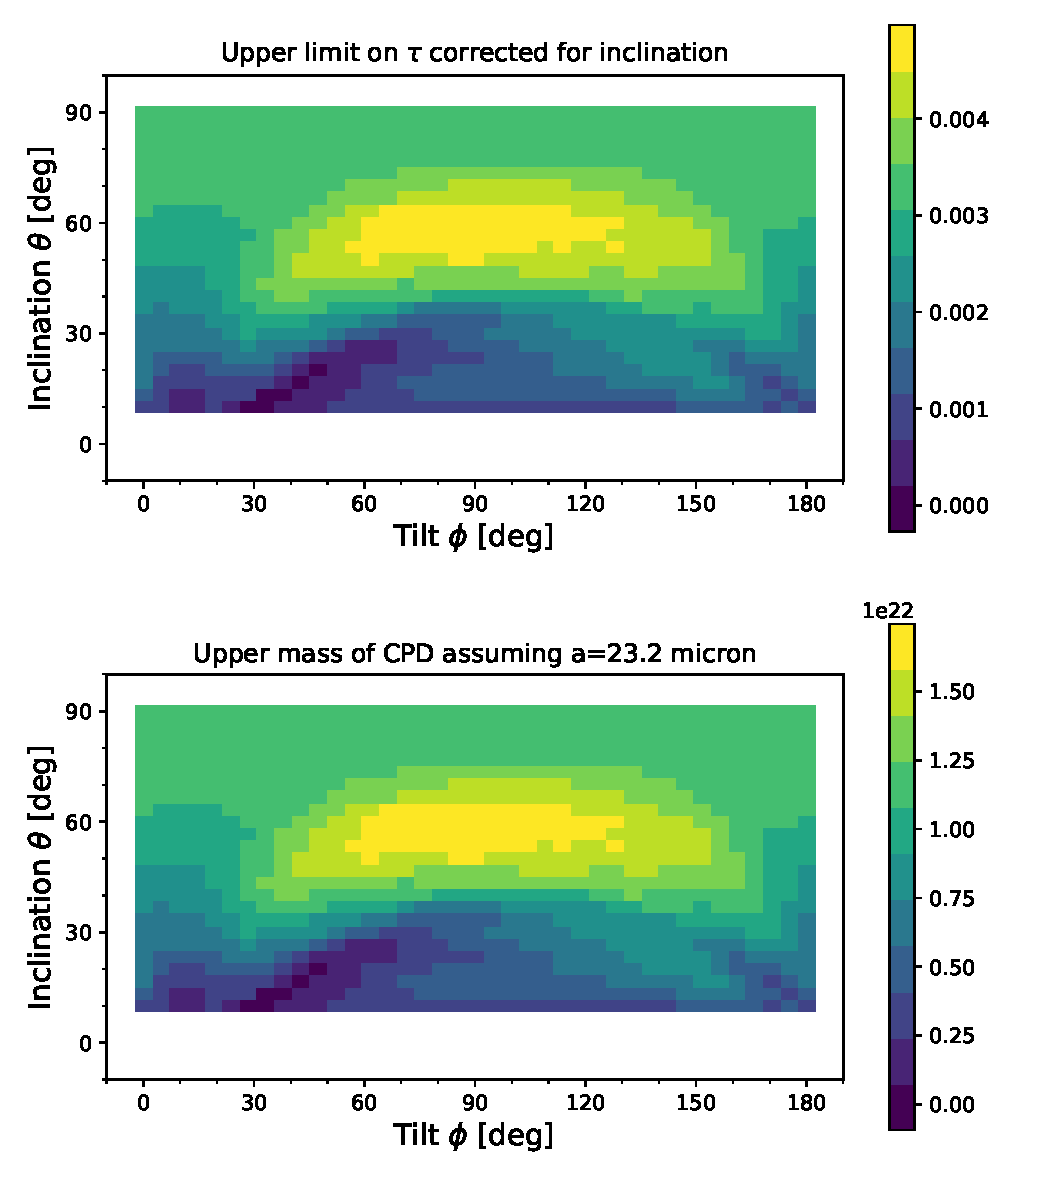
\includegraphics[width=0.50\textwidth]{diskfit_taumass_060.pdf}
    \caption{Circumplanetary disk  models for 0.30\rhill{} and  0.60\rhill{} radii. The upper row of each panel shows the $\tau$ corrected for disk inclination, and the lower panels show the upper limit on the total mass of the disk assuming mean particle sizes of $16.4\mu m$ and $23.2\mu m$.}
    \label{totalcpd}
\end{figure*}

%--------------------------------------------------------------------

\subsection{The 1981 event }

A significant photometric fluctuation was seen towards \bp{} around 1981 November 10 and subsequently reported in \citet{LecavelierdesEtangs95}.
%
This variation was seen in five separate colour filters in the optical bands and appeared to have no significant colour component \citep{Lamers97}.
%
Plausible models that could explain these photometric fluctuations include a horseshoe-shaped cloud of dust following an orbit of a (then hypothesized) gas giant planet \citep{LecavelierdesEtangs97} or the large tail of an evaporating falling body with a comet-like tail structure \citep{Lamers97}.
%
One possible explanation for the 1981 event is that it was generated by constructive interference of the $\delta$ Scuti pulsations from \bp{} itself; however, the observed pulsations of \bp{} can only constructively increase the total flux by $\sim$0.1\% over timescales of a few minutes, and, as such, we ruled out this explanation. Another explanation is that the event was a result of systematic errors in the original observations, but since the effect was observed simultaneously in several optical bands, this is considered highly unlikely \citep{LecavelierdesEtangs95}.
%
Although the photometry is relatively sparse, one simple model is forward scattering at small angles from a cloud of small particles that do not directly block the disk of the star, combined with a much shorter duration transit event that brings the flux back to the nominal level of starlight.

The light curve is shown in Fig.~\ref{fig:1981model} with a simple forward scattering model fitted to the measured photometry, as described in \citet{Lamers97}.
%
An astrometric fit by \citet{Wang16} showed that the planet does not transit the star and so is not responsible for the 1981 event.
%
Instead, we considered whether a circumplanetary ring could be responsible for the 1981 event, where an optically thick, narrow ring sits within a broader optically thin ring.
%
This ring is centred on \bpb{}, and since the radius of the ring is much larger than the diameter of the star, the segment of the circumplanetary ring that crosses the stellar disk can be approximated by a straight line.
%
We followed \citet{Lamers97} and modelled the 1981 event as a Gaussian with a full width at half maximum of 3.2 days and an amplitude of 0.035 magnitudes to model forward scattering from the optically thin part of the ring as well as with a notch feature representing the optically thick part of the ring, shown in Fig.~\ref{fig:1981model}, such that the model $F_{1981}(t)$ has the midpoint of the model at $t=0$.
%
We then fitted the photometry of \bp{} to ascertain if we could see a similar ring transit feature during the transit.

\begin{figure}[htb]
\centering
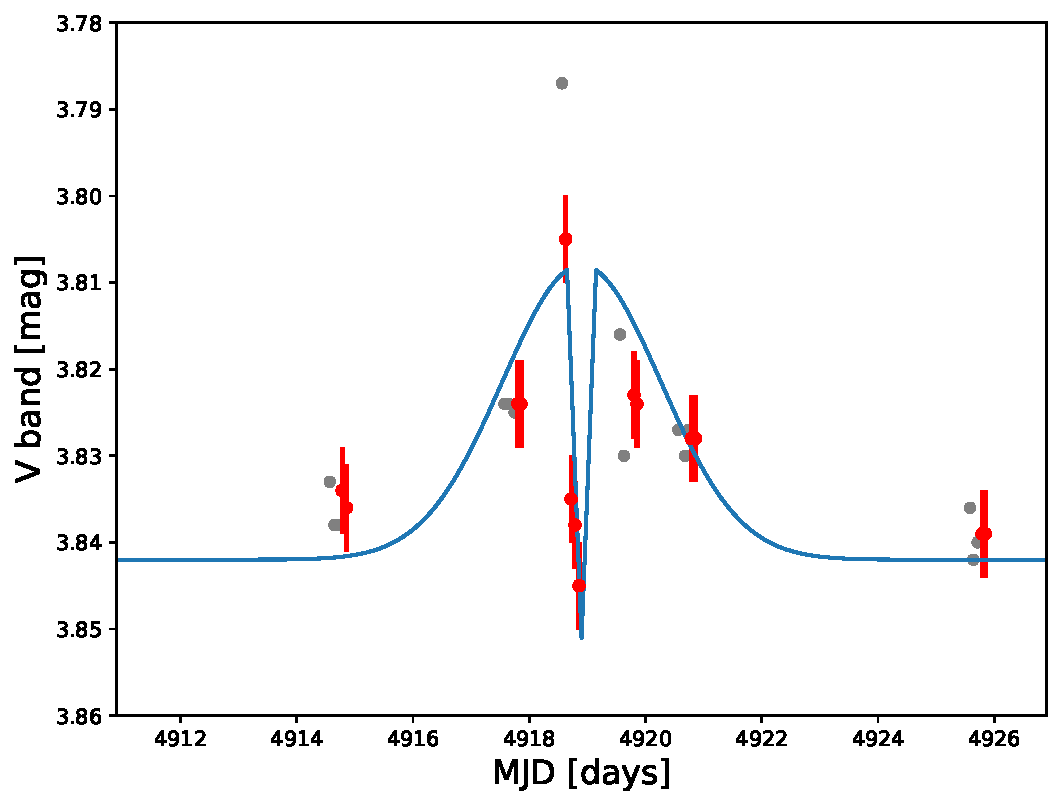
\includegraphics[width=\columnwidth]{m1981model.pdf}
\caption{Model for the 1981 event. The grey photometric points are V band magnitudes reported in \citet{LecavelierdesEtangs95}, and the red points the subset of the photometry that passed quality checks from that paper. The red error bars were reported in \citet{Lamers97}, and the parameters for the model (shown in blue) were derived from those reported in Fig. 7 of \citet{Lamers97}.}
\label{fig:1981model}
\end{figure}

For each telescope, we chose a test epoch $t_{mid}$ for the midpoint of the 1981 model and then fitted a two-parameter model:

$$F(t) = a F_{1981}(t_{mid}) + b,$$

where $a$ and $b$ are free parameters.
%
The parameter $a$ is the amplitude of the model, and $b$ is a constant offset in flux that accounts for any long-term trends in the photometry from the star and telescope systematics.
%
A non-linear fitting routine then takes a trial value of $t_{mid}$ and returns the best fit values of $a$ and $b$ for each test epoch.
%
The parameter $t_{mid}$ was chosen from MJD 58700 to 58200 in steps of 1 day.
%
The routine returns $a$ and its error, and the results for all three telescopes are shown in the upper panel of Fig.~\ref{fig:1981fit}.
%
As for the CPD fitting, each telescope is treated separately, represented by the different colour points and error bars on $a$.
%
The dotted line represents an amplitude $a$ that is consistent with the 1981 event.
%
The trial time $t_{mid}$ is ruled out if the amplitude $a$ and its error bar do not reach the 1981 event level at $a=0.035$.

Due to the systematic errors in the ground-based observatories, the fitted parameters do not always agree with each other within their respective error bars.
%
Under the hypothesis that there is no 1981 transit event in the Hill sphere of \bpb,{} we took the lower of the two determined values of $a$, resulting in the lower panel of Fig.~\ref{fig:1981fit}.
%
There are a few trial days where no model fit is determined due to a lack of data, with the longest gap being around 57920.
%
The fits on days adjacent to these gaps are consistent with no 1981 event, so we consider it highly unlikely that a transit event was missed.
%
On MJD 57942 the error bar from bRing was larger than 0.04, meaning that it does not rule out a 1981 transit event, but the two days to either side of this event are significantly inconsistent with a 1981 event.
%
We therefore conclude that there was no 1981 transit-like event during any part of the passage of the Hill sphere of \bpb{}.

\begin{figure*}[htb]
\centering
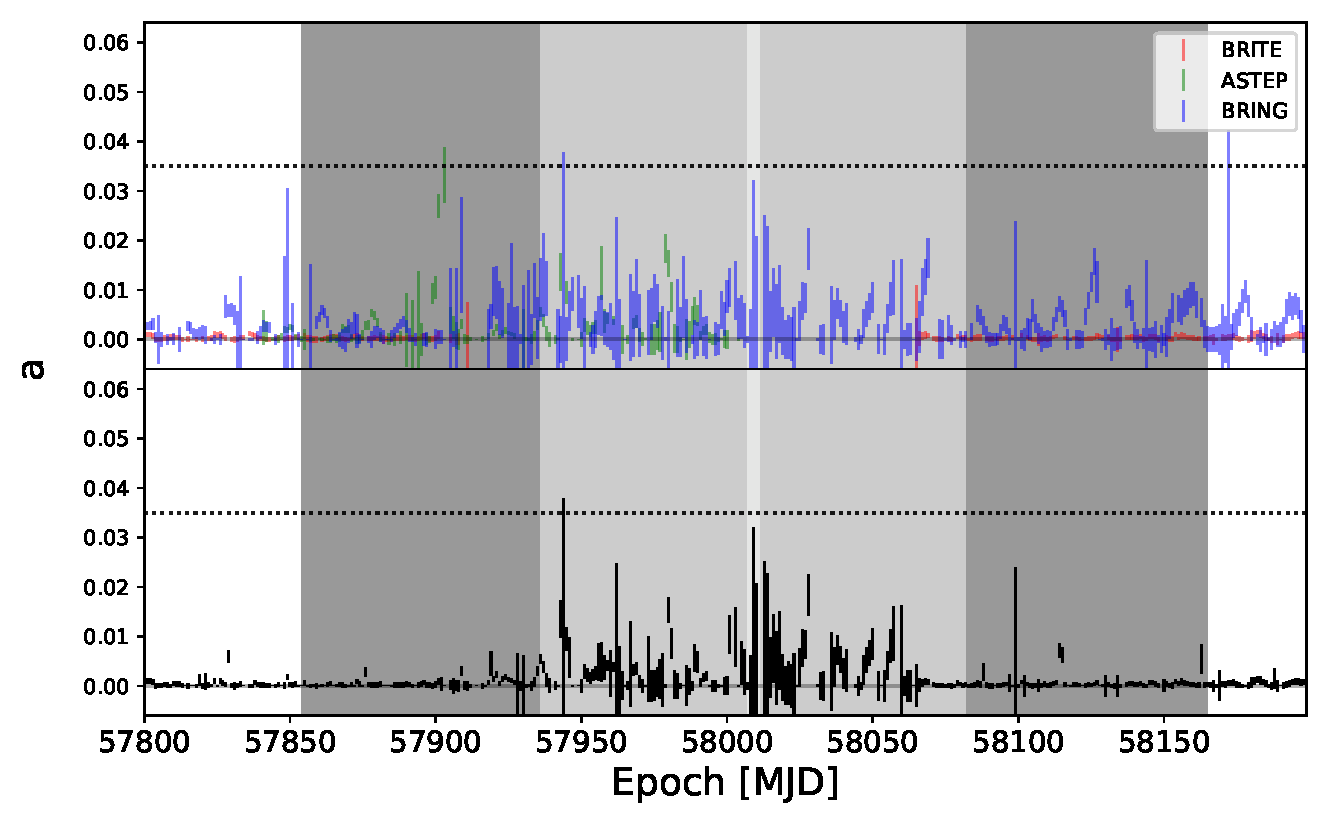
\includegraphics[width=0.9\linewidth]{fit_to_1981_model.pdf}
\caption{Result of fitting the 1981 model light curve (shown in Fig.~\ref{fig:1981model}) to the data from BRITE, ASTEP, and bRing. The upper panel shows the value of the fit amplitude $a$, and the dotted line shows the measured amplitude from the 1981 event. The error bars are one sigma limits determined from the {\tt lmfit} algorithm. The lower panel shows the smallest value of $a$ if there is more than one telescope with data. The dark grey and light grey panels indicate the 100\% and 50\% radii of the Hill sphere, respectively.}
\label{fig:1981fit}
\end{figure*}

\section{Discussion and conclusions }\label{sec:concl}

This paper presents the first photometric monitoring campaign of the Hill sphere of a gas giant exoplanet beyond the ice line of the host star.
%
Several observing campaigns led by different research groups have combined their data to provide continuous coverage of the $\sim 300$ day duration of the transit, making this analysis possible.
%
We detect no signal consistent with a \ac{cpd} crossing the line of sight within the Hill sphere, placing an upper limit of $1.8\times 10^{22}g$ on any possible \ac{cpd} under our detection limits.
%
There are several interpretations to our results:
\begin{enumerate}
    \item There is a dust disk that has a projected radius smaller than 10\% of the Hill sphere radius, so it does not transit the star.
    \item There is a larger dust disk that has a low obliquity and does not transit the star.
    \item There are no significant amounts $(<1.8\times 10^{22}g)$ of circumplanetary micron-sized dust in the Hill sphere.
\end{enumerate}

%
The coplanarity of moons around the gas giants in our Solar System implies the existence of CPDs at earlier epochs, and, given the large amount of dust in the \bp{} system, it is almost certain that there must have been a \ac{cpd} around \bpb{}.
%
We conclude that the circumplanetary dust has already condensed into moons, that it is in the form of a disk with a projected radius smaller than 10\% of the Hill radius, or that there is a CPD below the sensitivity limit of our observations.
% Mass estimate from Perez+ 2019: 1.2e+24 g
This is corroborated by ALMA observations that place upper limits on all the millimetre-sized dust in the Hill sphere of the planet \citep{Perez192}.
%
Our upper mass limit is more than 60 times smaller than the limit placed by ALMA observations.

A transit event in 1981 was hypothesized to be due to a circumstellar clump of material, an exocomet tail, or a narrow ring associated with a planet.
%
Our temporal coverage and photometric precision rules out a similar transit event, and so we conclude that the 1981 event was not due to dust in the circumplanetary environment of \bpb{}.
%
Whether the 1981 event was a singular, transitory event within the \bp{} system or was a long-lived structure associated with one of the planets within the system remains to be seen.
%
The 1981 transit event remains unexplained.
%
We are continuing to monitor \bp{} with the bRing stations in South Africa and Australia to see if we detect any material at the L3 and L4 Lagrange points in 2022.
%
The announcement of a second planet, \bp{} c, with a six-year orbital period, introduces the possibility of a second Hill sphere transit that we can monitor for rings or other circumplanetary material.

It is reasonable to assume that there are other Hill sphere transits around young stars, and we continue our searches in both archival data and in Evryscope and Transiting Exoplanet Survey Satellite (TESS) data, using second Gaia data release proper motions to identify pre-main-sequence stars ($<20Myr$) for candidates.
%
The ultimate goal is to identify a Hill sphere transit from archival photometric observations, plan a high time cadence spectrophotometric campaign where the circumplanetary environment of a forming gas giant planet and its attendant moons can be studied, and determine their physical and chemical compositions.
%
Hill sphere transits remain an exciting prospect for studying spatial and spectral scales of circumplanetary environments that cannot be investigated using other imaging techniques.

\section{Source code}
We are committed to open science and have made the data, reduction scripts, and plots in this paper available on an open source basis.
%
They are available at \url{https://github.com/mkenworthy/beta_pic_b_hill_sphere_transit}.
%
All code is provided under a Berkeley Software Distribution (BSD) 2-Clause `Simplified' license.

%--------------------------------------------------------------------


\begin{acknowledgements}

  We thank the referee for taking the time to review our paper, especially after the difficulties and disruptions of the past year.
  %
  MAK acknowledges funding from NOVA and Leiden Observatory for the bRing observatory at SAAO, and to the NSF/NWO for travel funding (NWO grant 629.003.025).
  %
  JW is supported by the 51 Pegasi b Fellowship.
  %
GMK is supported by the Royal Society as a Royal Society University Research Fellow.
  %
  MAK thanks the staff and observatory support crews at the South African Astronomical Observatory in Sutherland for all the work they put in to make bRing a successful observing station, and which allowed us to obtain first light within the first week of installation.
  %
  Part of this research was carried out at the Jet Propulsion Laboratory, California Institute of Technology, under a contract with the National Aeronautics and Space Administration (80NM0018D0004).
%
Construction of the bRing observatory sited at Siding Springs, Australia was made possible with a University of Rochester University Research Award, help from Mike Culver and Rich Sarkis (UR), and generous donations of time, services, and materials from Joe and Debbie Bonvissuto of Freight Expediters, Michael Akkaoui and his team at Tanury Industries, Robert Harris and Michael Fay at BCI, Koch Division, Mark Paup, Dave Mellon, and Ray Miller and the Zippo Tool Room.
%
The results reported herein benefitted from collaborations and/or information exchange within NASA’s Nexus for Exoplanet System Science (NExSS) research coordination network sponsored by NASA’s Science Mission Directorate.
  %
  This research is based on observations made with the NASA/ESA Hubble Space Telescope obtained from the Space Telescope Science Institute, which is operated by the Association of Universities for Research in Astronomy, Inc., under NASA contract NAS 5–26555. These observations are associated with programs 14621 and 15119.
%
ASTEP benefited from the support of the French and Italian polar agencies IPEV and PNRA in the framework of the Concordia station program and of Idex UCAJEDI (ANR-15-IDEX-01).
%
This research made use of Astropy,\footnote{http://www.astropy.org} a community-developed core Python package for Astronomy \citep{astropy:2013, astropy:2018}, Python \citep{vanRossum95,Oliphant07}, Matplotlib \citep{Hunter07,Caswell20},
% thomas_a_caswell_2020_4030140
numpy \citep{Oliphant06,vanderWalt11} and SciPy \citep{Virtanen20,Virtanen20B}.
% pauli_virtanen_2020_4100507}.

\end{acknowledgements}

%-------------------------------------------------------------------

\bibliographystyle{aa}
\bibliography{bpic_hill}

\newpage

\end{document}
